% Nota técnica: geometria do folheto Wheatley de dois círculos (versão 2, português do Brasil; tradução de main.tex).
% \claim{C-xxx} marca a afirmação registrada como C-xxx em CLAIMS.md (repositório); não imprime nada e aparece no Apêndice A.
\documentclass[11pt,a4paper]{article}
\usepackage[utf8]{inputenc}
\usepackage[T1]{fontenc}
\usepackage[brazil]{babel}
\usepackage{amsmath,amssymb,amsthm}
\usepackage{newtxtext,newtxmath}
\usepackage{microtype}
\usepackage{graphicx,booktabs,xcolor,longtable,array}
\usepackage[margin=2.4cm,top=2.6cm,bottom=2.6cm]{geometry}
\usepackage{fancyhdr}
\usepackage{titlesec}
\usepackage{enumitem}
\usepackage[font=small,labelfont=bf,margin=1em,justification=justified]{caption}
\usepackage[round,authoryear]{natbib}
\usepackage{pgfplots}
% Shared style of the figures (TikZ/pgfplots). Data: figures/data/, generated by sim/scripts/technote_figures.py.
\usepgfplotslibrary{fillbetween,groupplots}
\usetikzlibrary{calc}
\pgfplotsset{compat=1.18}
\definecolor{sone}{HTML}{2A78D6}
\definecolor{stwo}{HTML}{E0662C}
\definecolor{ink}{HTML}{161616}
\definecolor{inktwo}{HTML}{4A4A48}
\definecolor{muted}{HTML}{8A8984}
\definecolor{faint}{HTML}{D4D3CC}
\definecolor{rtwo}{HTML}{9CC3F2}
\definecolor{rthree}{HTML}{2A78D6}
\definecolor{rfour}{HTML}{1C5CAB}
\definecolor{rfive}{HTML}{104281}
\definecolor{rsix}{HTML}{0B3263}
\definecolor{rseven}{HTML}{0B2447}
\newcommand{\figdata}{figures/data/}
% generated by sim/scripts/technote_figures.py
\def\ptconCone{(-0.30000,0.00000)}
\def\ptconCtwo{(0.35000,-0.60622)}
\def\ptconE{(-1.00000,0.00000)}
\def\ptconP{(0.50000,-0.86603)}
\def\ptconM{(0.32911,-0.30695)}
\def\ptconO{(0.00000,0.00000)}
\def\ptconTh{(-0.16500,-0.28579)}
\def\ptsecMzero{(0.49606,-0.77738)}
\def\ptsecMone{(0.46132,-0.59058)}
\def\ptsecMtwo{(0.38462,-0.39970)}
\def\ptsecMthree{(0.26214,-0.21861)}
\def\ptsecMfour{(0.09635,-0.06330)}
\def\ptsecMfive{(0.00000,-0.00000)}
\def\ptflatonetop{(0.94349,0.78091)}
\def\ptflatoneJ{(1.02802,1.80834)}
\def\ptflatonebase{(1.97602,1.04658)}
\def\ptflattwotop{(0.94349,0.78091)}
\def\ptflattwoJ{(0.34267,0.60278)}

% generated by sim/scripts/technote_figures.py: label positions on the renders (fractions)
\def\labAVone{0.2572,0.9298}
\def\labAVtwo{0.5396,0.0222}
\def\labAM{0.5379,0.4804}
\def\labAE{0.2572,0.1801}
\def\labBO{0.5000,0.7347}
\def\aspectA{1.2674}
\def\aspectB{1.2500}

\pgfplotsset{
  geom/.style={axis equal image, hide axis, clip=false, scale only axis},
  graph/.style={axis lines=left, clip=false, scale only axis,
    axis line style={inktwo, line width=0.5pt}, tick style={inktwo, line width=0.4pt},
    tick label style={font=\footnotesize, text=inktwo}, label style={font=\small},
    every axis plot/.append style={line width=0.9pt}},
  every axis plot/.append style={line join=round},
  every axis/.append style={unbounded coords=jump},
}
\tikzset{
  dot/.style={circle, fill=ink, inner sep=0pt, minimum size=3.2pt},
  odot/.style={circle, draw=#1, fill=white, line width=0.6pt, inner sep=0pt, minimum size=3.4pt},
  lab/.style={font=\small, text=ink, inner sep=1.5pt},
  halo/.style={fill=white, fill opacity=0.85, text opacity=1, rounded corners=1pt, inner sep=1.2pt},
  panel/.style={font=\small\bfseries, text=ink},
}

\pgfkeys{/pgf/number format/.cd, use comma, 1000 sep={}}
\definecolor{linkblue}{RGB}{31,78,140}
\definecolor{taggray}{RGB}{110,110,110}
\usepackage[colorlinks=true,linkcolor=linkblue,citecolor=linkblue,urlcolor=linkblue]{hyperref}
\usepackage[capitalise,noabbrev]{cleveref}
\setlist{itemsep=2pt,topsep=4pt}
\setlength{\emergencystretch}{3em}
\titleformat{\section}{\large\bfseries}{\thesection}{0.6em}{}
\titleformat{\subsection}{\normalsize\bfseries}{\thesubsection}{0.6em}{}
\titlespacing*{\section}{0pt}{16pt}{6pt}
\titlespacing*{\subsection}{0pt}{10pt}{4pt}
\titleformat{\paragraph}[runin]{\normalsize\bfseries}{}{}{}
\pagestyle{fancy}
\fancyhf{}
\fancyhead[L]{\small\textcolor{taggray}{Geometria do folheto Wheatley de dois círculos}}
\fancyhead[R]{\small\textcolor{taggray}{B.~B.~Trigueiro}}
\fancyfoot[C]{\small\thepage}
\renewcommand{\headrulewidth}{0.3pt}
\theoremstyle{plain}
\newtheorem{theorem}{Teorema}[section]
\newtheorem{proposition}[theorem]{Proposição}
\newtheorem{lemma}[theorem]{Lema}
\newtheorem{corollary}[theorem]{Corolário}
\theoremstyle{remark}
\newtheorem{remark}[theorem]{Observação}
\crefname{theorem}{Teorema}{Teoremas}
\crefname{proposition}{Proposição}{Proposições}
\crefname{lemma}{Lema}{Lemas}
\crefname{corollary}{Corolário}{Corolários}
\crefname{remark}{Observação}{Observações}
\crefname{section}{Seção}{Seções}
\crefname{subsection}{Seção}{Seções}
\crefname{appendix}{Apêndice}{Apêndices}
\crefname{figure}{Figura}{Figuras}
\crefname{table}{Tabela}{Tabelas}
\crefname{equation}{}{}
\crefname{enumi}{item}{itens}
\newcommand{\crefpairconjunction}{ e }
\newcommand{\crefmiddleconjunction}{, }
\newcommand{\creflastconjunction}{ e }
\newcommand{\claim}[1]{\ifcsname claimseen@#1\endcsname\else\expandafter\gdef\csname claimseen@#1\endcsname{}\label{claim:#1}\fi}
\newcommand{\R}{\mathbb{R}}
\newcommand{\repourl}{\url{https://github.com/koobzaar/wheatley-two-circle-geometry}}

\title{\bfseries Sobre a geometria do folheto Wheatley de dois círculos}
\author{Bruno Bezerra Trigueiro\\[2pt]
  \small Instituto de Ciências Matemáticas e de Computação (ICMC)\\
  \small Universidade de São Paulo (USP), São Carlos, SP, Brasil}
\date{Nota técnica \quad Setembro de 2026}

\begin{document}
\maketitle
\thispagestyle{fancy}

\begin{abstract}
\noindent Estudamos a geometria dos folhetos da construção de dois círculos de \citet{McKee2026} e a sua extensão natural
para $N$ folhetos. Três resultados podem ser úteis aos autores desse artigo.
\begin{enumerate}[label=(\roman*),leftmargin=2em]
\item \emph{A junção é uma quina.} As duas metades de cada folheto se encontram com um ângulo de dobra de $41$--$47^\circ$
  ($49$--$53^\circ$ com as proporções dos modelos de $15$\,mm do artigo). Para $N\ge3$ os dois cones não admitem nenhuma
  junção com plano tangente contínuo; só $N=2$ não tem quina.
\item \emph{Comparar diferentes $N$ exige fixar alguma coisa.} Com a área total dos folhetos fixa, fixar o raio do anel ou a
  altura dá formas diferentes; igualar a área total do desenho linear com $N=3$ fixando os dois é impossível para $N=4$
  (certificado) e $N=5,6,7$ quando $H=R$. Nas duas famílias de área igual com o perfil linear do artigo, o maior ângulo de
  dobra cresce com $N$ para $N=2,\dots,7$.
\item \emph{Folhas planas.} Cada metade de um folheto é um pedaço de cone e pode ser cortada de uma folha plana (damos os
  moldes), mas o folheto inteiro com $N=3$ (na normalização do artigo) não, nem mesmo com uma dobra curva ao longo da
  junção. Isso só importa para a fabricação a partir de folha plana.
\end{enumerate}
Uma comparação exploratória por elementos finitos entre a junção com quina e uma junção arredondada não sustenta nenhuma
conclusão mecânica. Todo resultado tem uma prova escrita ou um método numérico declarado; identidades algébricas e resultados
geométricos selecionados estão, além disso, formalizados em Lean~4/mathlib, como indica o Apêndice~A.

\medskip\noindent\textbf{Palavras-chave:} superfícies desenvolvíveis; cones; dobras curvas; folhetos de válvula cardíaca;
válvulas poliméricas; verificação formal.\\
\textbf{MSC 2020:} 53A05, 92C10, 68V20.
\end{abstract}

\tableofcontents

%======================================================================
\section{Introdução}\label{sec:intro}

A válvula de Wheatley reforçada é uma válvula aórtica polimérica de três folhetos cuja forma, na construção de
\citet{McKee2026}, é gerada por duas famílias de círculos: em cada altura $z$, a seção de um folheto é um arco de um círculo
grande seguido de um arco de um círculo pequeno. Os dois círculos principais são tangentes internamente numa comissura; um arco
do círculo grande e um arco do círculo pequeno girado por $2\pi/3$ se encontram num ponto de junção $M(z)$ e formam um folheto
(\cref{fig:construction}). A construção é explícita, e os autores tiram dela uma
comparação de desenhos e um estudo por elementos finitos. Numa palestra no ICMC-USP (setembro de 2026), o grupo propôs
comparar válvulas com diferentes números de folhetos, $N\in\{2,\dots,7\}$. Esta nota estuda a geometria da construção com
duas perguntas práticas em mente: como comparar valores diferentes de $N$ de forma justa, e se um folheto pode ser cortado de
uma folha plana de polímero.

\paragraph{Contribuições.}
\begin{itemize}
\item Cada metade de um folheto é um pedaço de um cone circular oblíquo (\cref{thm:cone}); logo, é desenvolvível e pode ser
  cortada plana e curvada na posição sem esticar. Damos os moldes planos (\cref{thm:flat}).
\item O folheto inteiro com $N=3$ não é desenvolvível, nem mesmo como uma dobra curva ao longo da junção, porque as curvaturas
  geodésicas das duas metades não coincidem ali (\cref{thm:notflat}).
\item A junção é uma quina, com ângulo de dobra de $41$--$47^\circ$ (\cref{thm:fold3}); para $N\ge3$ os dois cones não têm
  plano tangente comum, de modo que não existe junção deles com plano tangente contínuo (\cref{thm:nocommon}).
\item A relação $a+b=1$ da construção não depende de $N$; as bordas livres fecham e, para todo $N$, as projeções cobrem o
  orifício com multiplicidade um em quase todo ponto (\cref{sec:N,sec:area,prop:cover}).
\item Para comparar $N$ com área total dos folhetos igual, a área escala como $R^2A^{\mathrm{tot}}_N(H/R,g)$, em que $g$ é o
  perfil vertical; igualar a área do desenho linear com $N=3$ mantendo $R$ e $H$ fixos é impossível para $N=4,\dots,7$ quando
  $H=R$, e as famílias de área igual com $R$ fixo ou com $H$ fixo estão tabeladas (\cref{sec:compare}).
\end{itemize}
Um repositório que acompanha a nota traz as provas em Lean, o código e um pacote com as famílias de área igual
(Disponibilidade dos dados).

\paragraph{Relação com trabalhos anteriores.}\claim{C-022} \citet{McKee2021} construíram um modelo anterior da válvula a
partir de círculos que se cruzam e se tocam. Eles observaram que o modelo tem linhas nos folhetos onde a derivada salta, e
argumentaram que a válvula dispensa molde porque a superfície de cada par de arcos é ``topologically equivalent to a laminar
sheet''. \citet{Rebolledo2023} removeram esse \emph{kink} com um trecho cúbico, em cada seção horizontal, entre os dois pontos
de interseção de um círculo grande com um pequeno. A construção de 2026 tem a mesma estrutura da de 2021 (um par de círculos
principais tangentes internamente sobre o círculo unitário, \citealp[eqs.~(5)--(6)]{McKee2021}, e uma junção onde cópias
giradas se encontram), com raios diferentes: $a+b=1$ em 2026, enquanto os raios $(1+b+b^2)/(2+b)$ e $(1-b)/2$ dos círculos de
2021 \citep[eqs.~(3.2)--(3.3)]{Rebolledo2023} somam $1+b(b-1)/(2(b+2))<1$ para $0<b<1$. A curva de junção $M$ de 2026 é,
portanto, o análogo do \emph{kink} de 2021, e a sua existência não é novidade. \citet{Oliveira2022} generalizaram o modelo de
2021 para elipses e mostraram folhetos desdobrados sobre um plano (p.~21 e Figs.~11--13 do artigo), e \citet{Oliveira2024}
afirmam que, para a fabricação, o folheto deveria poder ser obtido recortando uma figura de uma folha plana de polímero e
dobrando-a na posição. O que é novo aqui, para a construção de 2026, é o valor da quina, a prova de que os dois cones não
admitem junção com plano tangente contínuo (com um lema de rigidez local indicando que um arredondamento desenvolvível teria
de sair deles), e a resposta à pergunta da folha plana: cada metade pode ser cortada plana e curvada sem esticar, mas o
folheto inteiro não. Ser topologicamente uma folha não implica isso.

%======================================================================
\section{A construção de dois círculos}\label{sec:construction}

\subsection{Convenções e parametrização}
Seguimos a normalização do artigo: raio do anel $1$, altura $z\in[0,1]$, $b=z/2$, $a=1-b$ \citep[eq.~(29) e a prova da
Prop.~1]{McKee2026}. As rotações $R_\theta$ em torno do eixo $z$ são anti-horárias, $E=(-1,0,0)$ e $O$ é a origem. Para $N$
folhetos, seja $\theta=2\pi/N$; o artigo é o caso $N=3$. As duas peças do folheto $0$ são
\begin{align}
X_1(t,z) &= \big(-b+a\cos t,\ a\sin t,\ z\big) &&\text{(arco $EM$; artigo, eqs.~(38)--(39))},\label{eq:X1}\\
X_2(t,z) &= R_\theta\big(-a+b\cos t,\ b\sin t,\ z\big) &&\text{(arco $MP$; eqs.~(40)--(41) para $\theta=2\pi/3$)},\label{eq:X2}
\end{align}
ambas no domínio de parâmetros $\Omega=\{(t,z): 0\le z\le 1,\ \pi\le t\le t_M(z)\}$, em que $t_M(z)$ é o parâmetro do ponto
de junção $M(z)$ \emph{nos dois} círculos; para $N=3$,
\[ t_M(z)=2\pi-\arccos\frac{1+2b-2b^2}{2D},\qquad D=1-b+b^2 . \]
As formas com arco-seno (p.~5, Apêndice~A \texttt{plot1}) e com arco-cosseno (p.~6, \texttt{plot2}) de $t_M$ no artigo
coincidem \claim{C-005} (o \cref{thm:aplusb} dá $t_M$ para todo $N$). O folheto $k$ é
$R_{k\theta}\big(X_1(\Omega)\cup X_2(\Omega)\big)$; $P=R_\theta E$ é a comissura seguinte. A \cref{fig:construction} mostra a
construção. A nossa família de $N$ folhetos mantém os dois círculos principais tangentes em $E$ e gira o segundo por $2\pi/N$;
é uma generalização nossa, não do artigo. As Seções~\ref{sec:cones} e~\ref{sec:crease} tratam $N=3$, salvo indicação em
contrário.

\begin{figure}[t]\centering
% Figure: the two-circle construction. (a) one section, z = 0.6; (b) the sections of one leaflet as z grows.
\begin{tikzpicture}
\begin{axis}[geom, width=0.44\textwidth, xmin=-1.12, xmax=1.12, ymin=-1.08, ymax=1.08, name=A]
  \addplot[muted, dashed, line width=0.45pt] table {\figdata ring.dat};
  \addplot[faint, line width=1.5pt] table {\figdata c_others.dat};
  \addplot[sone, densely dotted, line width=0.55pt] table {\figdata c_big.dat};
  \addplot[stwo, densely dotted, line width=0.55pt] table {\figdata c_small.dat};
  \addplot[sone, line width=2.1pt, line cap=round] table {\figdata c_arc1.dat};
  \addplot[stwo, line width=2.1pt, line cap=round] table {\figdata c_arc2.dat};
  \addplot[inktwo, line width=0.5pt] table {\figdata c_theta.dat};
  \draw[muted, line width=0.45pt] \ptconO -- \ptconE  \ptconO -- \ptconP;
  \draw[sone, line width=0.7pt] \ptconCone -- node[lab, above, text=sone] {$a$} \ptconE;
  \draw[stwo, line width=0.7pt] \ptconCtwo -- node[lab, right, text=stwo] {$b$} \ptconP;
  \node[odot=sone] at \ptconCone {};
  \node[odot=stwo] at \ptconCtwo {};
  \node[lab, text=inktwo] at \ptconTh {$\theta$};
  \node[dot] at \ptconO {}; \node[lab, anchor=south west] at \ptconO {$O$};
  \node[dot] at \ptconE {}; \node[lab, anchor=east] at \ptconE {$E$};
  \node[dot] at \ptconP {}; \node[lab, anchor=north west] at \ptconP {$P$};
  \node[dot] at \ptconM {}; \node[lab, anchor=north west, xshift=1pt, yshift=-1pt] at \ptconM {$M$};
  \node[panel, anchor=north west] at (rel axis cs:0,1) {(a)};
\end{axis}
\begin{axis}[geom, width=0.44\textwidth, xmin=-1.12, xmax=1.12, ymin=-1.08, ymax=1.08,
             at={($(A.east)+(0.06\textwidth,0)$)}, anchor=west]
  \addplot[muted, dashed, line width=0.45pt] table {\figdata ring.dat};
  \addplot[sone, line width=1pt, opacity=0.35] table {\figdata sec0_1.dat};
  \addplot[stwo, line width=1pt, opacity=0.35] table {\figdata sec0_2.dat};
  \addplot[sone, line width=1pt, opacity=0.48] table {\figdata sec1_1.dat};
  \addplot[stwo, line width=1pt, opacity=0.48] table {\figdata sec1_2.dat};
  \addplot[sone, line width=1pt, opacity=0.61] table {\figdata sec2_1.dat};
  \addplot[stwo, line width=1pt, opacity=0.61] table {\figdata sec2_2.dat};
  \addplot[sone, line width=1pt, opacity=0.74] table {\figdata sec3_1.dat};
  \addplot[stwo, line width=1pt, opacity=0.74] table {\figdata sec3_2.dat};
  \addplot[sone, line width=1pt, opacity=0.87] table {\figdata sec4_1.dat};
  \addplot[stwo, line width=1pt, opacity=0.87] table {\figdata sec4_2.dat};
  \addplot[sone, line width=2.1pt] table {\figdata sec5_1.dat};
  \addplot[stwo, line width=2.1pt] table {\figdata sec5_2.dat};
  \addplot[ink, line width=0.8pt] table {\figdata junction_top.dat};
  \node[dot, minimum size=2.6pt] at \ptsecMzero {};
  \node[dot, minimum size=2.6pt] at \ptsecMone {};
  \node[dot, minimum size=2.6pt] at \ptsecMtwo {};
  \node[dot, minimum size=2.6pt] at \ptsecMthree {};
  \node[dot, minimum size=2.6pt] at \ptsecMfour {};
  \node[dot] at \ptconO {}; \node[lab, anchor=south east] at \ptconO {$O$};
  \node[dot] at \ptconE {}; \node[lab, anchor=east] at \ptconE {$E$};
  \node[dot] at \ptconP {}; \node[lab, anchor=north west] at \ptconP {$P$};
  \node[lab, text=inktwo, anchor=south] at (axis cs:-0.5,0.02) {$z=1$};
  \node[panel, anchor=north west] at (rel axis cs:0,1) {(b)};
\end{axis}
\end{tikzpicture}

\caption{A construção de dois círculos ($N=3$). (a) Uma seção horizontal, $z=0{,}6$. A superfície~1 é o arco $EM$ do círculo
grande (centro $(-b,0)$, raio $a=1-b$; azul); a superfície~2 é o arco $MP$ do círculo pequeno (raio $b=z/2$) girado por
$\theta=2\pi/3$ em torno de $O$ (laranja). $E$ e $P=R_\theta E$ são comissuras e $M$ é a junção; pontilhado: os círculos
completos; cinza: as seções dos outros dois folhetos. (b) Seções de um folheto em $z=0{,}1;\,0{,}3;\dots;0{,}9$ (do claro ao
escuro) e a borda livre $z=1$ (grossa); a junção $M(z)$ (preto) vai de $P$, em $z=0$, a $O$, em $z=1$.}
\label{fig:construction}
\end{figure}

\paragraph{Escala vertical.} Os modelos mecânicos do artigo têm $20$\,mm de diâmetro e $15$\,mm de altura, enquanto
$z\in[0,1]$ com raio do anel $1$ dá altura de $10$\,mm para raio de $10$\,mm. As Seções~\ref{sec:cones}--\ref{sec:area}
usam a família normalizada (escala vertical $h=1$), salvo indicação em contrário; a \cref{sec:compare} trata $h=H/R$ geral.
Um esticamento vertical $(x,y,z)\mapsto(x,y,hz)$ preserva a estrutura cônica e a desenvolvibilidade, mas muda ângulos, áreas
e moldes planos (\cref{prop:vscale}).

\subsection{Observações sobre a fonte}\label{sec:source}
\claim{C-004}\claim{C-007}\claim{C-008}Ao transcrever as fórmulas das páginas renderizadas de \citet{McKee2026}, notamos três
pontos que os autores talvez queiram conhecer; nenhum afeta a construção.
\begin{enumerate}
\item A eq.~(28) como impressa, $\sin t=-\sqrt{a-b}/(2(a^2+ab+b^2))$, não é consistente com (27) e (29): com ela,
  $\cos^2t+\sin^2t-1=-(2b-1)(3b-1)/(2D^2)$ na família $a=1-b$, que só se anula em $b=1/3$ e $b=1/2$. A expressão pretendida
  é $-\sqrt3\,(a-b)/(2(a^2+ab+b^2))$, que reaparece nas pp.~5--6.
\item Com rotações anti-horárias, o ápice da segunda superfície é $V_2=(\tfrac12,-\tfrac{\sqrt3}{2},0)=P$, que é $X_2(t,0)$
  para todo $t$. A Proposição~1 imprime $(\tfrac12,+\tfrac{\sqrt3}{2},0)$, obtido aplicando (3)--(4) como mapa de pontos (uma
  rotação horária) a $(-1,0,0)$. O conjunto dos seis ápices em (54) é o mesmo nas duas leituras; só muda a atribuição dos
  ápices aos folhetos.
\item Na prova da Proposição~1, o passo ``$y=0$'' divide por $\sin t_j-\sin t_i$, que se anula para $t_i=4\pi/3$,
  $t_j=5\pi/3$ (ambos em $EM$). O enunciado continua verdadeiro (\cref{thm:cone}).
\end{enumerate}

%======================================================================
\section{Estrutura cônica e desenvolvibilidade}\label{sec:cones}

\begin{theorem}[Proposição~1 de \citealp{McKee2026}, reenunciada]\label{thm:cone}\claim{C-001}
Para todo $(t,z)\in\R^2$,
\[ X_1(t,z)=\big(1-\tfrac z2\big)(\cos t,\sin t,0)+\tfrac z2\, V_1,\qquad X_2(t,z)=\big(1-\tfrac z2\big)V_2+\tfrac z2\,Q(t), \]
com $V_1=(-1,0,2)$, $V_2=R_\theta E=P$ e $Q(t)=R_\theta(\cos t,\sin t,2)$, um ponto de um círculo unitário na altura $2$. Logo,
toda haste $t=\mathrm{const}$ da superfície $i$ está numa reta que passa por $V_i$: a superfície~1 é um pedaço do cone sobre o
círculo unitário com ápice $V_1$, e a superfície~2 um pedaço do cone sobre o círculo de $Q$ com ápice $V_2$.
\end{theorem}
\begin{proof}
Com $b=z/2$ e $a=1-b$, \eqref{eq:X1} fica $\big(-b+(1-b)\cos t,\,(1-b)\sin t,\,2b\big)=(1-b)(\cos t,\sin t,0)+b(-1,0,2)$. Em
\eqref{eq:X2}, $R_\theta$ é linear e fixa o eixo $z$, logo $X_2=R_\theta\big((1-b)(-1,0,0)+b(\cos t,\sin t,2)\big)
=(1-b)V_2+bQ(t)$. Para $t$ fixo, as duas expressões são afins em $z$, e $X_1(t,2)=V_1$, $X_2(t,0)=V_2$.
\end{proof}

As duas superfícies são, portanto, \emph{aplicações cônicas} $X(t,z)=V+(\alpha+\beta z)\,w(t)$:
\begin{equation}\label{eq:conemaps}
\begin{aligned}
X_1&=V_1+\big(1-\tfrac z2\big)w_1, & w_1(t)&=(\cos t+1,\ \sin t,\ -2),\\
X_2&=V_2+\tfrac z2\,w_2, & w_2(t)&=R_\theta(\cos t+1,\ \sin t,\ 2).
\end{aligned}
\end{equation}

\begin{lemma}[Aplicações cônicas]\label{lem:conemap}\claim{C-006}\claim{C-002}
Seja $X=V+(\alpha+\beta z)\,w(t)$ com $w$ de classe $C^2$. Então $X_t=(\alpha+\beta z)w'$, $X_z=\beta w$ e
$X_t\times X_z=(\alpha+\beta z)\beta\,(w'\times w)$. Logo, $X$ é uma imersão em $(t,z)$ se e somente se $\alpha+\beta z\ne0$,
$\beta\ne0$ e $w'(t)\times w(t)\ne0$, e em todo ponto assim a sua curvatura gaussiana $K=(LN-M^2)/(EG-F^2)$ se anula.
\end{lemma}
\begin{proof}
As derivadas são imediatas. Para $K$: $X_{zz}=0$, logo $N=0$; e $X_{tz}=\beta w'=\tfrac{\beta}{\alpha+\beta z}X_t$ é tangente,
logo $M=X_{tz}\cdot n=0$. Assim, $LN-M^2=0$.
\end{proof}

\begin{lemma}[Os dois cones do folheto]\label{lem:leafcones}
Para todo $\theta$, $c_1:=w_1'\times w_1=(-2\cos t,\,-2\sin t,\,-(1+\cos t))$ e
$c_2:=w_2'\times w_2=R_\theta(2\cos t,\,2\sin t,\,-(1+\cos t))$, com $|c_1|^2=|c_2|^2=4+(1+\cos t)^2>0$. Além disso,
$|w_i'|=1$ e $|w_i|^2=6+2\cos t\ge4$. Consequentemente, $X_1$ é regular se e somente se $z\ne2$ (logo em todo $\Omega$) e $X_2$
se e somente se $z\ne0$, e as duas têm $K\equiv0$ nos seus pontos regulares.
\end{lemma}
\begin{proof}
Cálculo direto; para $c_2$, use que uma rotação em torno do eixo $z$ comuta com o produto vetorial. A última frase segue do
\cref{lem:conemap} com $(\alpha,\beta)=(1,-\frac12)$ e $(0,\frac12)$.
\end{proof}

\begin{theorem}[Moldes planos]\label{thm:flat}\claim{C-010}
Sejam $r(t)=\sqrt{6+2\cos t}$ e
\[ \varphi(t)=\int_\pi^t\frac{\sqrt{4+(1+\cos s)^2}}{6+2\cos s}\,ds. \]
As aplicações planas $D_1(t,z)=(1-\tfrac z2)\,r(t)\,(\cos\varphi,\sin\varphi)$ e $D_2(t,z)=\tfrac z2\,r(t)\,(\cos\varphi,\sin\varphi)$
têm a mesma primeira forma fundamental que $X_1$ e $X_2$ em todo $(t,z)$; elas são imersões exatamente onde $X_1$, $X_2$ são
e, portanto, isometrias locais ali. $D_1$ é injetora em $\Omega$ e $D_2$ em $\Omega\cap\{z>0\}$, e todo ângulo de setor
$\varphi(t_M(z))$ está em $[0,\pi/2]$ (numericamente $0{,}8816$, $1{,}0539$ e $1{,}2526$\,rad em $z=0,\tfrac12,1$).
\end{theorem}
\begin{proof}
Para uma aplicação cônica com $r=|w|$ e $\varphi'=|w'\times w|/|w|^2$, ponha $D=(\alpha+\beta z)\,r\,e(\varphi)$,
$e=(\cos,\sin)$. Então $D_t=(\alpha+\beta z)(r'e+r\varphi'e^\perp)$ e $D_z=\beta r e$, de modo que
$E_D=(\alpha+\beta z)^2(r'^2+r^2\varphi'^2)$, $F_D=(\alpha+\beta z)\beta\,rr'$, $G_D=\beta^2r^2$, enquanto para $X$,
$E=(\alpha+\beta z)^2|w'|^2$, $F=(\alpha+\beta z)\beta\,w\cdot w'$, $G=\beta^2|w|^2$. Ora, $rr'=w\cdot w'$ e, pela identidade de
Lagrange, $r^2(r'^2+r^2\varphi'^2)=(w\cdot w')^2+|w'\times w|^2=|w|^2|w'|^2$; logo as duas formas coincidem, e também os
determinantes $EG-F^2$, o que prova a afirmação sobre imersões. Pelo \cref{lem:leafcones},
$\varphi'=|w'\times w|/|w|^2\le |w'|/|w|\le\frac12$ e $\varphi'>0$; como $t_M(z)-\pi\le\pi$, o ângulo de setor está em
$[0,\pi/2]$. Nesse setor $\varphi$ é estritamente crescente, de modo que o ângulo polar de $D(t,z)$ determina $t$, e então o
raio $(\alpha+\beta z)r(t)$ determina $z$ ($\beta\ne0$; $1-\frac z2>0$, e $\frac z2>0$ para $z>0$).
\end{proof}

Assim, cada metade pode ser cortada de uma folha plana e curvada na posição sem esticar (\cref{fig:flat}).

\begin{proposition}[Os dois cones são congruentes]\label{prop:congruent}\claim{C-009}
A isometria $T(x,y,z)=(R_\theta(x,y),\,2-z)$ satisfaz $T(X_1(t,z))=X_2(t,2-z)$ para todo $(t,z)$, e $T(V_1)=V_2$. Os segmentos
completos de haste $0\le z\le1$ com o mesmo $t$ têm o mesmo comprimento $\tfrac12\sqrt{6+2\cos t}$ nas duas superfícies.
Dentro de $\Omega$, esse é o comprimento da haste para $\pi\le t\le5\pi/3$; para $t$ maior, a haste começa na altura
$z_{\min}(t)$ em que $t_M(z_{\min})=t$, e o seu comprimento é $\tfrac12\sqrt{6+2\cos t}\,(1-z_{\min}(t))$ nas duas
superfícies. As duas \emph{peças} usadas no folheto não são congruentes: a superfície~1 usa a metade do seu cone longe do
ápice, a superfície~2 a metade junto a ele.
\end{proposition}
\begin{proof}
Trocar $z$ por $2-z$ troca $b$ por $1-b$, logo $X_2(t,2-z)=R_\theta\big(-b+(1-b)\cos t,\ (1-b)\sin t,\ 2-z\big)$, que é
$T(X_1(t,z))$; e $T(V_1)=(R_\theta(-1,0),0)=V_2$. Ao longo de uma haste, as duas aplicações são afins em $z$ com velocidade
$\frac12|w_i|=\frac12\sqrt{6+2\cos t}$ (\cref{lem:leafcones}), o que dá os dois comprimentos. Por fim, as duas peças têm
áreas diferentes: pelos \cref{lem:conemap,lem:leafcones},
$\mathrm{Área}(X_1(\Omega))-\mathrm{Área}(X_2(\Omega))=\frac12\int_\Omega(1-z)\sqrt{4+(1+\cos t)^2}\,dt\,dz>0$, de modo que
nenhuma isometria leva uma na outra.
\end{proof}

\begin{figure}[t]\centering
% Figure: the leaflet in 3D (PyVista renders; labels placed by the camera projection in leaflet3d_labels.tex).
\begin{tikzpicture}
\node[anchor=south west, inner sep=0] (a) at (0,0) {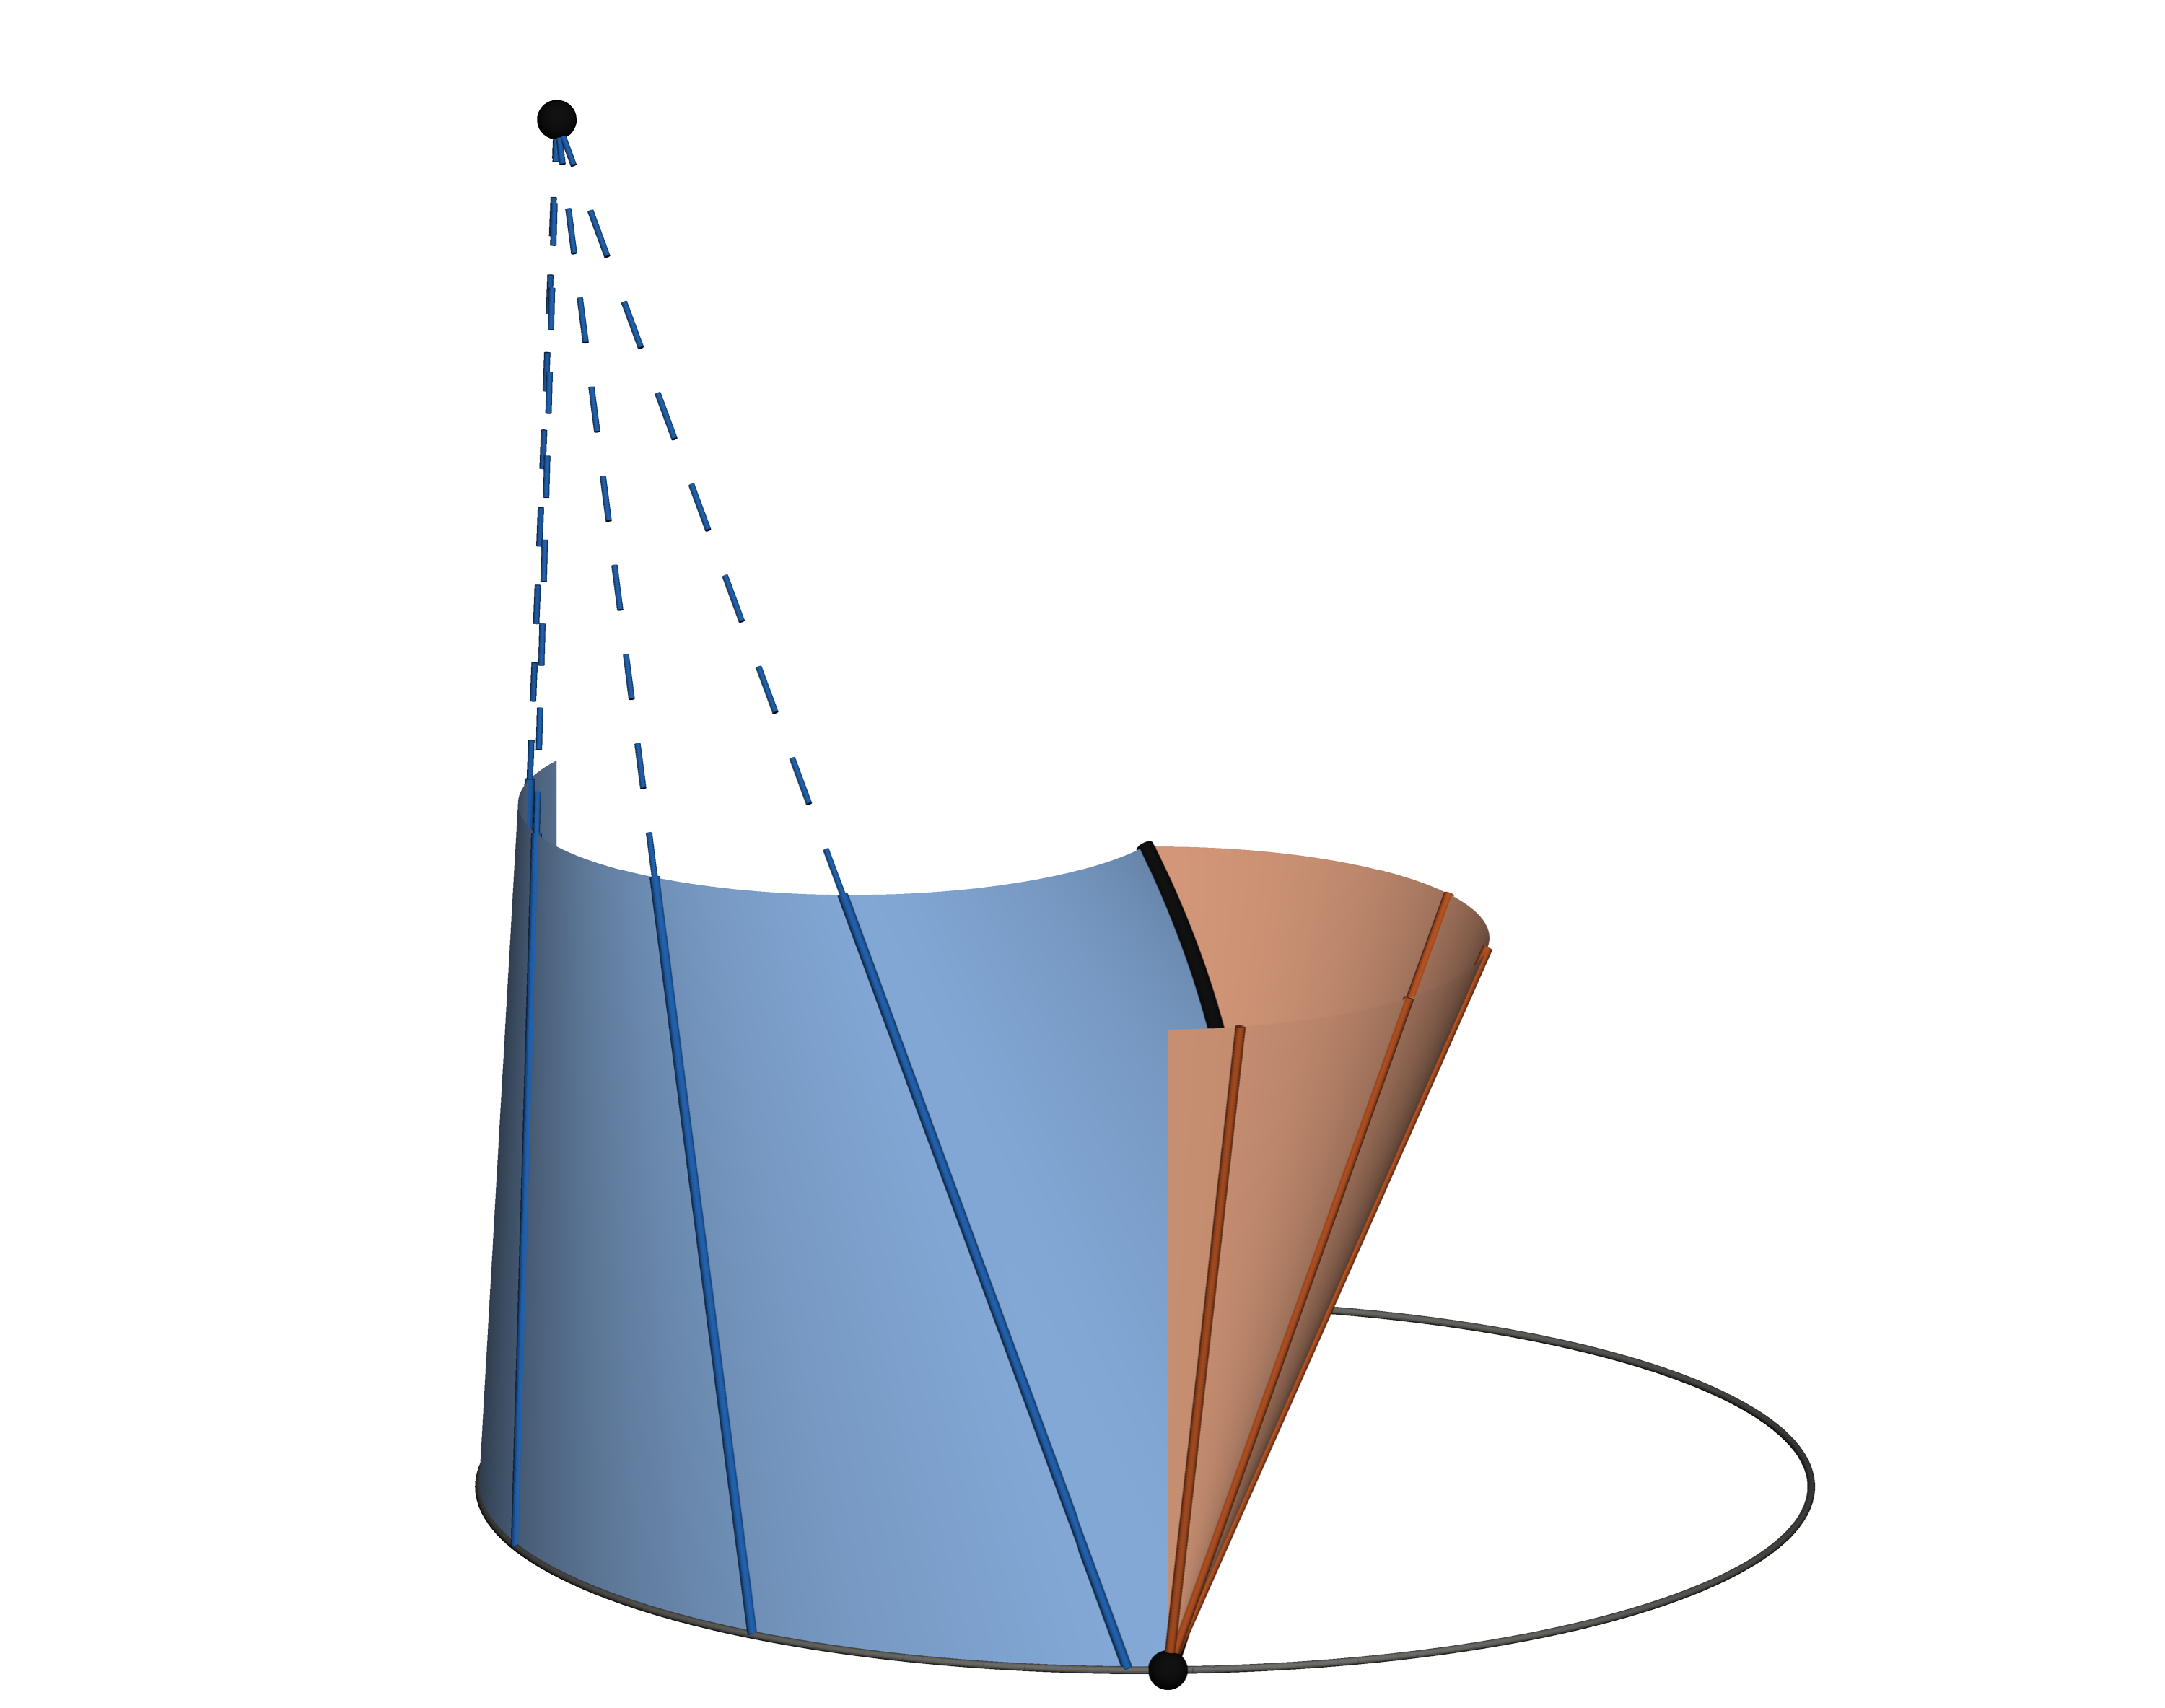
\includegraphics[width=0.43\textwidth]{figures/leaflet3d_a.png}};
\begin{scope}[x={(a.south east)}, y={(a.north west)}]
  \node[lab, anchor=west, xshift=3pt] at (\labAVone) {$V_1=(-1,0,2)$};
  \node[lab, anchor=north west, xshift=2pt] at (\labAVtwo) {$V_2=P$};
  \draw[inktwo, line width=0.4pt] (\labAM) -- ++(0.1,0.13) node[lab, anchor=south west, inner sep=1pt] {$M(z)$};
  \node[lab, anchor=east, xshift=-6pt] at (\labAE) {$E$};
  \node[panel, anchor=north west] at (0,1) {(a)};
\end{scope}
\node[anchor=south west, inner sep=0] (b) at ($(a.south east)+(0.1\textwidth,0)$)
  {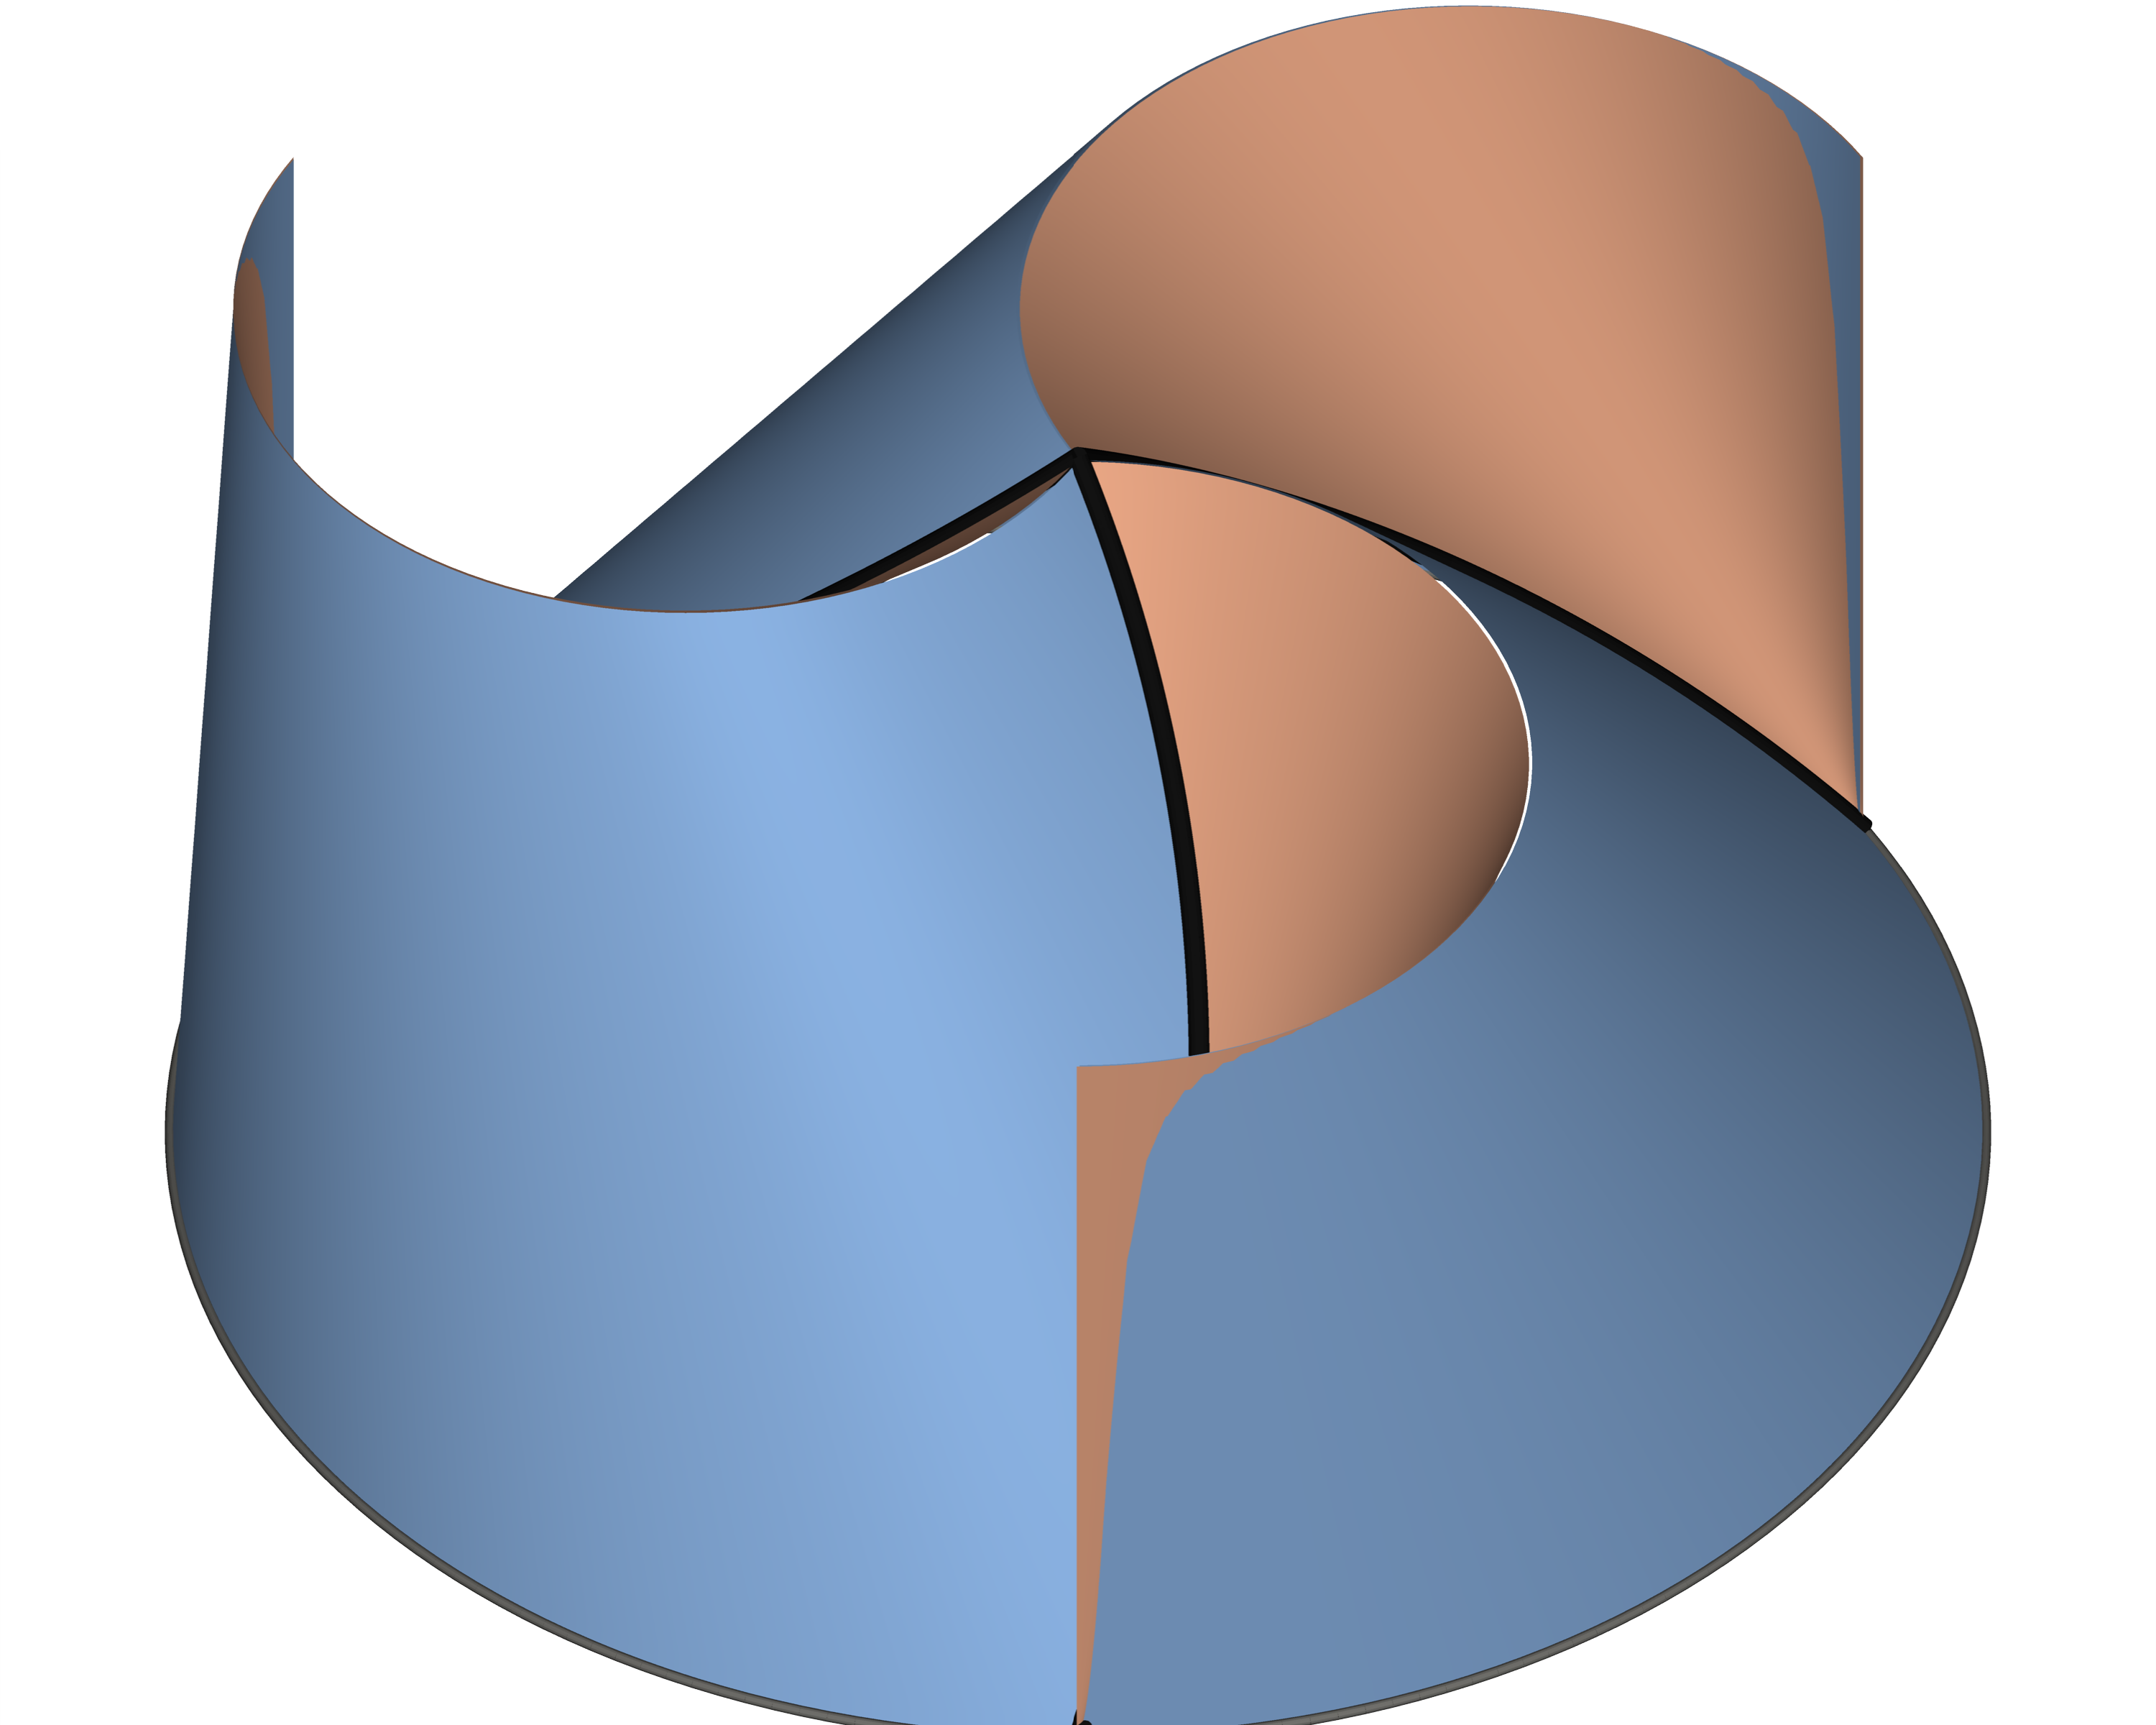
\includegraphics[width=0.43\textwidth]{figures/leaflet3d_b.png}};
\begin{scope}[shift={(b.south west)}, x={($(b.south east)-(b.south west)$)}, y={($(b.north west)-(b.south west)$)}]
  \node[lab, halo, anchor=south, yshift=3pt] at (\labBO) {$O$};
  \node[panel, anchor=north west] at (-0.08,1) {(b)};
\end{scope}
\end{tikzpicture}

\caption{(a) Um folheto ($N=3$). A superfície~1 (azul) é um pedaço do cone com ápice $V_1=(-1,0,2)$, acima da válvula: as suas
hastes (linhas azuis) se prolongam (tracejado) até $V_1$. A superfície~2 (laranja) é um pedaço do cone com ápice $V_2=P$, na
base do poste da comissura, de onde partem as suas hastes. Preto: a junção $M(z)$. (b) A válvula de três folhetos. Renderização
a partir da parametrização exata, com câmera ortográfica.}
\label{fig:leaflet}
\end{figure}

\begin{theorem}[O folheto inteiro não é desenvolvível]\label{thm:notflat}\claim{C-011}
Sejam $k_1,k_2$ as curvaturas geodésicas da junção $M(z)$ como curva na superfície~1 e na superfície~2, cada uma medida com a
conormal apontando para dentro da sua própria peça. Então
\[ k_1+k_2=\frac{4\sqrt3\,(z-1)\,\tilde D^2}{\sqrt{\tilde D^2+9}\,(\tilde D^2+12)^{3/2}},\qquad \tilde D=z^2-2z+4, \]
que é negativa para $0<z<1$ (valor $-5408\sqrt{939}/2146867$ em $z=\tfrac12$) e se anula em $z=1$. A curvatura gaussiana
concentrada carregada pela junção é $\int_M(k_1+k_2)\,ds\approx-0{,}10825$\,rad. Consequentemente, nenhuma vizinhança dos
dois lados de um ponto $M(z_0)$, $0<z_0<1$, no folheto é intrinsecamente isométrica a uma região plana: o folheto não pode
ser obtido de uma única folha plana por flexão e dobra sem esticar.
\end{theorem}
\begin{proof}
A fórmula de $k_1+k_2$ é um cálculo de álgebra computacional a partir de \eqref{eq:X1}--\eqref{eq:X2}, exato em alturas
racionais; ela coincide com as curvaturas das duas imagens da junção nos moldes planos, calculadas de forma independente
(\cref{fig:flat}c). Uma isometria preserva a curvatura geodésica das curvas \citep[prova do seu teorema
principal]{FuchsTabachnikov1999}. Suponha que uma vizinhança dos dois lados de $M(z_0)$, onde as duas peças e a junção são
regulares, fosse intrinsecamente isométrica a uma região plana. Então um arco de $M$ em torno de $M(z_0)$ seria levado numa
única curva plana, com as duas peças em lados opostos dela; logo $k_1=-k_2$ ao longo desse arco, o que contradiz $k_1+k_2<0$
em $(0,1)$. (Em $z=1$, $k_1+k_2=0$ num único ponto, o que não prova nada; $z=0$ é singular.) Equivalentemente, por
Gauss--Bonnet, duas peças planas coladas ao longo de uma curva formam uma superfície intrinsecamente plana perto dessa curva
só se $k_1+k_2=0$.
\end{proof}

Cada metade, porém, pode ser cortada plana (\cref{thm:flat}). Dobrar também não resolve: uma folha curvada e dobrada sem
esticar continua intrinsecamente plana, e $k_1+k_2=0$ ao longo do vinco é a condição que os dois lados de uma dobra curva de
uma única folha têm de satisfazer \citep{FuchsTabachnikov1999}; em particular, o folheto não é uma dobra curva ao longo de $M$.
Nos moldes planos, as duas imagens da junção têm o mesmo comprimento ($1{,}44932$) mas curvaturas diferentes, de modo que não
podem ser costuradas borda com borda no plano. Isso diz respeito apenas à fabricação a partir de uma folha plana, a via
mencionada por \citet{Oliveira2024}; moldagem ou imersão (\emph{dip-casting}) não são afetadas. O passo de Gauss--Bonnet é
clássico e não está formalizado.

\begin{figure}[t]\centering
% Figure: flat patterns of the two halves (true stays, t = const) and the curvature of the two images of the junction.
\begin{tikzpicture}
\begin{axis}[geom, width=0.3\textwidth, name=A]
  \addplot[sone, line width=0.45pt] table {\figdata flat1_z.dat};
  \addplot[sone, line width=0.45pt] table {\figdata flat1_stays.dat};
  \addplot[sone, line width=1.3pt] table {\figdata flat1_base.dat};
  \addplot[sone, line width=1.3pt] table {\figdata flat1_top.dat};
  \addplot[ink, line width=1.8pt] table {\figdata flat1_junction.dat};
  \node[lab, text=sone, anchor=west, xshift=2pt] at \ptflatonebase {$z=0$};
  \node[lab, text=sone, anchor=east, xshift=-2pt] at \ptflatonetop {$z=1$};
  \node[lab, anchor=south east, xshift=-1pt, yshift=1pt] at \ptflatoneJ {$M$};
  \node[panel, anchor=south west] at (rel axis cs:0,1.02) {(a)};
\end{axis}
\begin{axis}[geom, width=0.17\textwidth, at={($(A.east)+(0.05\textwidth,0)$)}, anchor=west, name=B]
  \addplot[stwo, line width=0.45pt] table {\figdata flat2_z.dat};
  \addplot[stwo, line width=0.45pt] table {\figdata flat2_stays.dat};
  \addplot[stwo, line width=1.3pt] table {\figdata flat2_top.dat};
  \addplot[ink, line width=1.8pt] table {\figdata flat2_junction.dat};
  \node[dot] at (axis cs:0,0) {};
  \node[lab, anchor=north east] at (axis cs:0,0) {$V_2$};
  \node[lab, text=stwo, anchor=west, xshift=2pt] at \ptflattwotop {$z=1$};
  \node[lab, anchor=east, xshift=-2pt] at \ptflattwoJ {$M$};
  \node[panel, anchor=south west] at (rel axis cs:0,1.02) {(b)};
\end{axis}
\begin{axis}[graph, width=0.27\textwidth, height=0.24\textwidth, at={($(B.east)+(0.17\textwidth,0)$)}, anchor=west,
             xmin=0, xmax=1, xlabel={$z$},
             legend style={draw=none, fill=none, font=\footnotesize, at={(0.98,0.03)}, anchor=south east},
             legend cell align=left]
  \addplot[sone, name path=kone] table {\figdata kg1.dat};
  \addplot[stwo, name path=ktwo] table {\figdata kg2neg.dat};
  \addplot[faint, forget plot] fill between[of=kone and ktwo];
  \legend{$k_1$, $-k_2$}
  \node[panel, anchor=south west] at (rel axis cs:-0.28,1.02) {(c)};
\end{axis}
\end{tikzpicture}

\caption{Moldes planos (a) da superfície~1 e (b) da superfície~2 (\cref{thm:flat}); as linhas finas são imagens de
$z=\mathrm{const}$ e das hastes ($t=\mathrm{const}$), e em preto está a imagem da junção $M$. (c) Curvatura geodésica da junção
de cada lado, medida em direção à própria peça, calculada a partir dos moldes planos. Costurar os dois moldes ao longo de $M$
exigiria $k_1=-k_2$; a faixa sombreada é $-(k_1+k_2)>0$ e coincide com a forma fechada do \cref{thm:notflat} até $10^{-4}$.}
\label{fig:flat}
\end{figure}

%======================================================================
\section{A junção é uma quina}\label{sec:crease}

As duas peças ficam do mesmo lado $t\le t_M$ da junção; por isso, uma orientação coerente do folheto inverte a normal de uma
delas. Definimos o ângulo de dobra $\delta$ como o ângulo entre $X_{1,t}\times X_{1,z}$ e $-(X_{2,t}\times X_{2,z})$:
$\delta=0$ significa continuidade do plano tangente.

\begin{lemma}[Ângulo de dobra num parâmetro comum]\label{lem:foldt}
Para todo $\theta$ e $0<z<2$, em pontos das duas superfícies com o mesmo parâmetro $t$,
\[ \cos\delta=\frac{(1+\cos t)^2-4\cos\theta}{4+(1+\cos t)^2}. \]
\end{lemma}
\begin{proof}
Pelo \cref{lem:conemap}, $X_{1,t}\times X_{1,z}=-\frac12(1-\frac z2)\,c_1$ e $-(X_{2,t}\times X_{2,z})=-\frac12\cdot\frac z2\,c_2$;
os dois fatores são negativos para $0<z<2$, de modo que $\delta$ é o ângulo entre $c_1$ e $c_2$. Pelo \cref{lem:leafcones},
$c_1\cdot c_2=-4\,(\cos t,\sin t)\cdot R_\theta(\cos t,\sin t)+(1+\cos t)^2=(1+\cos t)^2-4\cos\theta$ e
$|c_1||c_2|=4+(1+\cos t)^2$.
\end{proof}

\begin{theorem}[Ângulo de dobra, $N=3$]\label{thm:fold3}\claim{C-003}
Para $0<z\le1$,
\[ \cos\delta(z)=\frac{8D^2+9}{16D^2+9},\qquad D=1-\tfrac z2+\tfrac{z^2}4, \]
logo $17/25\le\cos\delta\le3/4$, isto é, $41{,}41^\circ\le\delta\le47{,}16^\circ$, com o mínimo na borda livre. O folheto é
$C^0$ mas não $G^1$ ao longo de toda a junção.
\end{theorem}
\begin{proof}
Na junção, $1+\cos t_M=1+\frac{1+2b-2b^2}{2D}=\frac{3}{2D}$ e $\cos\theta=-\frac12$, de modo que o \cref{lem:foldt} dá
$\cos\delta=\big(\frac{9}{4D^2}+2\big)/\big(\frac{9}{4D^2}+4\big)=\frac{8D^2+9}{16D^2+9}$. A função $u\mapsto(8u+9)/(16u+9)$ é
decrescente, e $D^2\in[\frac9{16},1]$ para $b\in[0,\frac12]$, com $D=\frac34$ em $z=1$; isso dá as cotas. Como $\cos\delta<1$
em todo ponto, os planos tangentes nunca coincidem ao longo de $M$, enquanto as duas peças se encontram ao longo de $M$
(\cref{thm:aplusb}).
\end{proof}

\begin{proposition}[Escala vertical]\label{prop:vscale}\claim{C-021}
Com escala vertical $h>0$ (a altura multiplicada por $h$), ao longo da junção do folheto com $N=3$, para $0<z\le1$,
\[ \cos\delta_h=\frac{8h^2D^2+9}{16h^2D^2+9}; \]
para $h=1{,}5$ ele varia em $[49{,}17^\circ;\,53{,}13^\circ]$ em vez de $[41{,}41^\circ;\,47{,}16^\circ]$.
\end{proposition}
\begin{proof}
O esticamento troca $w_1,w_2$ por $(\cos t+1,\sin t,-2h)$ e $R_\theta(\cos t+1,\sin t,2h)$, logo $c_1,c_2$ por
$(-2h\cos t,-2h\sin t,-(1+\cos t))$ e $R_\theta(2h\cos t,2h\sin t,-(1+\cos t))$, e a prova do \cref{lem:foldt} dá
$\cos\delta_h=((1+\cos t)^2-4h^2\cos\theta)/(4h^2+(1+\cos t)^2)$. Substitua $1+\cos t_M=3/(2D)$ e $\cos\theta=-\frac12$, e
avalie a expressão monótona em $D=\frac34$ e $D=1$.
\end{proof}

A quina pode ser arredondada mantendo o folheto desenvolvível, para que ele ainda possa ser formado a partir de material
plano? Os dois cones não podem ser ligados diretamente um ao outro (\cref{thm:nocommon} e a observação em seguida); para um
arredondamento ao longo de uma faixa, temos apenas um lema local e uma expectativa, enunciados a seguir.

\begin{theorem}[Não há plano tangente comum]\label{thm:nocommon}\claim{C-017}
Para $N\ge3$, os dois cones não têm plano tangente comum: não existem hastes $t_1,t_2$ cujos planos tangentes coincidam. Para
$N=2$, as hastes $t_1=t_2=2\pi$, que formam a junção, compartilham o plano tangente.
\end{theorem}
\begin{proof}
Pelo \cref{lem:conemap}, o plano tangente do cone $i$ ao longo da haste $t$ é o plano que passa por $V_i$ com normal $c_i(t)$
(a haste inteira está nele). Os planos de $t_1$ e $t_2$ coincidem se e somente se $c_1(t_1)\parallel c_2(t_2)$ e
$(V_2-V_1)\cdot c_1(t_1)=0$. Um cálculo dá $(V_2-V_1)\cdot c_1(t_1)=2\,(1+\cos(t_1-\theta))$, logo $t_1\equiv\theta+\pi$ e
$c_1(t_1)=(2\cos\theta,\,2\sin\theta,\,-(1-\cos\theta))$. As partes horizontais de $c_1(t_1)$ e $c_2(t_2)$ têm ambas
comprimento $2$, de modo que ser paralelo significa $c_2(t_2)=\pm c_1(t_1)$. Com o sinal $+$, as partes horizontais dão
$t_2\equiv0$ e as verticais $-2=-(1-\cos\theta)$, isto é, $\cos\theta=-1$; com o sinal $-$, $t_2\equiv\pi$ e $0=1-\cos\theta$,
isto é, $\cos\theta=1$. Nenhum dos dois vale para $N\ge3$. Para $N=2$, $\theta=\pi$ e $t_1=t_2\equiv0$ satisfazem as duas
condições.
\end{proof}

Um cone tem o mesmo plano tangente ao longo de toda uma haste. Num ponto onde uma peça do cone~1 encontra uma peça do cone~2
com continuidade do plano tangente, o plano tangente comum seria tangente ao cone~1 ao longo de uma haste e ao cone~2 ao longo
de uma haste. Logo, para $N\ge3$, \emph{não} existe junção $G^1$ entre os dois cones, ao longo de nenhuma curva.

\begin{lemma}[Rigidez local; clássico]\label{lem:rigid}\claim{C-018}
Seja $S$ uma superfície regular de classe $C^\infty$ com $K\equiv0$. Suponha que $S$ contenha uma peça aberta $C_0$ de um
cone, longe do seu ápice, tal que a segunda forma fundamental $\mathrm{II}$ do cone nunca se anule em $C_0\cup\gamma$, e seja
$\gamma\subset S$ uma curva no interior de $S$ que limita $C_0$ e é transversal às hastes. Então, perto de cada ponto interior
de $\gamma$, $S$ coincide com esse cone.
\end{lemma}
A hipótese $\mathrm{II}\ne0$ não pode ser retirada: um cone não plano pode conter regiões planas, e uma superfície desenvolvível
pode sair do cone por uma delas.\footnote{O gráfico de $y\,\varphi(x/y-1)$, com $\varphi(s)=e^{-1/s^2}$ para $s>0$ e
$\varphi(s)=0$ para $s\le0$, é um cone não plano que é plano onde $x<y$; em $|x|<1/4$ ele é plano para $1/2<y<1$ e é
continuado, para $1\le y<3/2$, pelo gráfico de $\varphi(y-1)$.} Para os dois cones do folheto ela vale em todo ponto regular:
$X_{tt}=(\alpha+\beta z)w''$, de modo que o coeficiente $tt$ de $\mathrm{II}$ é um múltiplo não nulo de $w''\cdot(w'\times w)$,
que vale $2$ para $w_1$ e $-2$ para $w_2$; os outros dois coeficientes se anulam (\cref{lem:conemap}). Logo $\mathrm{II}\ne0$
para $z\ne2$ na superfície~1 e $z\ne0$ na superfície~2.
\begin{proof}
Usamos dois fatos clássicos para superfícies lisas com $K\equiv0$ \citep[\S5-8, Proposições~1 e~2, devidas a
Massey]{doCarmo1976}: por um ponto parabólico (onde $K=0$ e $\mathrm{II}\ne0$) passa uma única linha assintótica, que é um
segmento aberto de reta ao longo do qual a normal unitária, e portanto o plano tangente, é constante; e um tal segmento
maximal nunca encontra um ponto planar. Como $S$ é lisa e coincide com o cone em $C_0$, a sua segunda forma fundamental num
ponto $q\in\gamma$ é, por continuidade a partir de $C_0$, a do cone em $q$, que é não nula por hipótese (para os cones do
folheto, $q$ está numa haste que entra em $C_0$ por transversalidade, longe do ápice, onde $L\ne0$); por continuidade, todo
ponto de $S$ perto de $q$ é parabólico e o campo de direções assintóticas é contínuo ali. A linha assintótica de $S$ por um
ponto de $C_0$ é a haste do cone por esse ponto (unicidade); assim, as hastes são segmentos retos de $S$ que cruzam $\gamma$.
Seja $r\in S$ perto de $q$, do outro lado de $\gamma$. O seu segmento assintótico é reto, com direção próxima da direção da
haste por $q$, e se estende até sair de uma vizinhança fixa de $q$ no interior de $S$ (ele não pode terminar num ponto
planar). Como $\gamma$ é transversal às hastes, o segmento cruza $\gamma$ num ponto $q'$ perto de $q$, onde tem de coincidir
com a haste por $q'$. Logo $r$ está no prolongamento de uma haste, isto é, no cone.
\end{proof}
A hipótese de suavidade vem da referência. Há versões para regularidade menor \citep[por exemplo,][]{HartmanNirenberg1959},
mas não conferimos as hipóteses exatas delas.

\begin{remark}[Esperado, não provado]\label{rem:expected}
Esperamos que, para $N\ge3$, nenhuma superfície desenvolvível $C^\infty$ coincida com o folheto fora de uma faixa estreita em
torno da junção $M$ (restrita a alturas $z$ num subintervalo compacto de $(0,1)$). Pelo \cref{lem:rigid}, as hastes dos dois
cones continuariam como retas dentro da faixa, e onde uma haste continuada de um cone alcançasse a outra peça os dois planos
tangentes teriam de coincidir, o que o \cref{thm:nocommon} exclui. Tornar isso preciso exige controlar onde as hastes
continuadas saem da faixa; não fizemos isso.
\end{remark}

\paragraph{Um arredondamento $G^1$.}\claim{C-019} Em cada seção horizontal $0<z\le1$, troca-se uma vizinhança de $M$ pelo arco
de círculo de raio $\rho(z)=\rho_0 z$ tangente aos dois círculos da seção. Cada seção fica então $G^1$ e a família varia
suavemente com $z$; logo a superfície é $G^1$. A faixa arredondada não é desenvolvível: numericamente, $K$ chega a cerca de
$-38$ (unidades normalizadas, $\rho_0=0{,}05$), e para $\rho_0=0{,}1$ é não nula em todas as amostras, com $\max|K|>1$. Isso é
coerente com a \cref{rem:expected}. A comparação mecânica da \cref{sec:fem} usa uma variante com raio
$\sqrt{(\rho_0z)^2+(T/R)^2}$ (nunca mais fina que a casca), que é suave em $z$, e remove o canto na base do poste da
comissura, onde o arredondamento não pode ser engrossado. Para $N=2$, a junção é uma haste comum com plano tangente comum
(\cref{thm:foldN}), e nenhum arredondamento é necessário. \citet{Oliveira2024} relatam flexão dos folhetos perto do centro na
diástole para a geometria de 2021; se uma quina deste tipo tem papel nisso não é tratado nesta nota.

%======================================================================
\section{$N$ folhetos}\label{sec:N}

\begin{theorem}[A relação $a=1-b$ não depende de $N$]\label{thm:aplusb}\claim{C-012}
Seja $\cos\theta\ne1$. Se o círculo grande $\{(a-1+a\cos t,\ a\sin t)\}$ e o círculo pequeno $\{(b-1+b\cos t,\ b\sin t)\}$
girado por $\theta$ têm um ponto em comum com o mesmo parâmetro $t$ nos dois, então $a+b=1$. Suponha além disso $0<\theta\le\pi$
(verdadeiro para $\theta=2\pi/N$), $0\le b\le\frac12$ e $a=1-b$. Então as duas superfícies se encontram no mesmo parâmetro
\[ t_M^\theta=2\pi-\arccos\frac{2ab-(a^2+b^2)\cos\theta}{\Delta},\qquad \Delta=a^2+b^2-2ab\cos\theta>0, \]
que é igual a $t_M$ para $N=3$. A junção vai de $t_M^\theta=\pi+\theta$, $M=R_\theta E$, em $z=0$, até $t_M^\theta=2\pi$, $M=O$, em $z=1$.
\end{theorem}
\begin{proof}
Escreva $e=(1,0)$, $u=(\cos t,\sin t)$ e $v=e+u$. Os dois pontos são $p=av-e$ e $q=bv-e$, e $p=R_\theta q$, logo $|p|=|q|$.
Como $|sv-e|^2=1-s(1-s)|v|^2$, isso dá $(a-b)(1-a-b)|v|^2=0$. Se $v=0$, então $p=q=-e$ e $-e=R_\theta(-e)$ força
$\cos\theta=1$, o que está excluído. Se $a=b$, então $p=q=R_\theta p$, logo $p=0$, isto é, $av=e$; daí $\sin t=0$,
$\cos t=1$, $v=2e$ e $a=b=\frac12$. Em todos os demais casos, $a+b=1$.

Para a junção, note primeiro que $\Delta=(a-b)^2+2ab(1-\cos\theta)>0$ para $b\in[0,\frac12]$, $a=1-b$ e
$\cos\theta<1$ (se $b=0$, então $\Delta=1$). Sejam $c=(2ab-(a^2+b^2)\cos\theta)/\Delta$ e $s=(b^2-a^2)\sin\theta/\Delta$. Com $a=1-b$, verifica-se que
$c^2+s^2=1$ e que \eqref{eq:X1} e \eqref{eq:X2} coincidem em $(\cos t,\sin t)=(c,s)$. Para $0<\theta\le\pi$ e $b\le\frac12$,
$s\le0$, logo $t=2\pi-\arccos c\in[\pi,2\pi]$. Em $z=0$ ($a=1$, $b=0$), $(c,s)=(-\cos\theta,-\sin\theta)$, logo $t=\pi+\theta$
e $M=(\cos(\pi+\theta),\sin(\pi+\theta))=R_\theta E$; em $z=1$ ($a=b=\frac12$), $(c,s)=(1,0)$, logo $t=2\pi$ e $M=O$. Para
$\theta=2\pi/3$, $c=(1+2b-2b^2)/(2D)$, o valor do artigo.
\end{proof}

\begin{theorem}[Ângulo de dobra para $N$ folhetos]\label{thm:foldN}\claim{C-014}
Para $0<z\le1$, ao longo da junção, com $X=1+\cos t_M^\theta=(1-\cos\theta)/\Delta$,
\[ \cos\delta=\frac{X^2-4\cos\theta}{X^2+4}. \]
Logo, a junção é uma quina se e somente se $\cos\theta\ne-1$, isto é, para todo $N\ge3$. Para $N=2$, a junção é a haste comum
$t=2\pi$ e o folheto é $G^1$. Na borda livre, $\cos\delta=\sin^2(\pi/N)$.
\end{theorem}
\begin{proof}
Com $a+b=1$, $1+c=\big((a^2+b^2)(1-\cos\theta)+2ab(1-\cos\theta)\big)/\Delta=(1-\cos\theta)/\Delta$; substitua isso no
\cref{lem:foldt}. Então $\cos\delta<1$ se e somente se $\cos\theta>-1$. Para $\theta=\pi$, $c=1$ para todo $z$, logo
$t_M\equiv2\pi$ e $\cos\delta=1$. Em $z=1$, $\Delta=\frac12(1-\cos\theta)$ e $X=2$, logo
$\cos\delta=(1-\cos\theta)/2=\sin^2(\theta/2)$.
\end{proof}

\begin{figure}[t]\centering
% Figure: fold angle along the junction, N = 2..7 (h = 1), and N = 3 with h = 1.5.
\begin{tikzpicture}
\begin{axis}[graph, width=0.55\textwidth, height=0.42\textwidth, xmin=0, xmax=1, ymin=-6, ymax=132,
             ytick={0,30,60,90,120}, xlabel={$z$}, ylabel={$\delta$ ($^\circ$)}]
  \addplot[rtwo] table {\figdata fold2.dat} node[pos=0.02, anchor=south west, inner sep=1pt, font=\footnotesize, text=muted] {$N=2$};
  \addplot[rthree, line width=1.4pt] table {\figdata fold3.dat} node[pos=0.55, anchor=north, inner sep=2pt, font=\footnotesize, text=rthree] {$N=3$};
  \addplot[rfour] table {\figdata fold4.dat} node[pos=0.02, anchor=south west, inner sep=1pt, font=\footnotesize, text=rfour] {$N=4$};
  \addplot[rfive] table {\figdata fold5.dat} node[pos=0.02, anchor=south west, inner sep=1pt, font=\footnotesize, text=rfive] {$N=5$};
  \addplot[rsix] table {\figdata fold6.dat} node[pos=0.02, anchor=south west, inner sep=1pt, font=\footnotesize, text=rsix] {$N=6$};
  \addplot[rseven] table {\figdata fold7.dat} node[pos=0.02, anchor=south west, inner sep=1pt, font=\footnotesize, text=rseven] {$N=7$};
  \addplot[rthree, dashed] table {\figdata fold3_h15.dat}
    node[pos=0.55, anchor=south, font=\footnotesize, text=rthree, yshift=1pt] {$N=3,\ h=\pgfmathprintnumber{1.5}$};
\end{axis}
\end{tikzpicture}

\caption{Ângulo de dobra $\delta$ ao longo da junção para $N=2,\dots,7$ (escala vertical $h=1$, \cref{thm:foldN}) e para
$N=3$ com $h=1{,}5$ (tracejado, \cref{prop:vscale}). Para $N\ge5$ a dobra passa de $90^\circ$ perto da base; para $N=2$ não há
quina.}
\label{fig:fold}
\end{figure}

\begin{theorem}[As bordas livres fecham para todo $N$]\label{thm:freeedge}\claim{C-013}
Em $z=1$, $X_2(t,1)=R_\theta X_1(t,1)$ para todo $t$: a segunda peça do folheto $k$ coincide ponto a ponto com a primeira peça
do folheto $k+1$. As bordas livres são $N$ semicírculos de raio $\frac12$ que ligam o centro às comissuras (\cref{fig:top}).
\end{theorem}
\begin{proof}
Em $z=1$, $a=b=\frac12$, de modo que tanto \eqref{eq:X1} quanto o argumento de $R_\theta$ em \eqref{eq:X2} valem
$(-\frac12+\frac12\cos t,\ \frac12\sin t,\ 1)$, o círculo de raio $\frac12$ centrado em $(-\frac12,0,1)$; $t\in[\pi,2\pi]$
percorre a metade que vai de $E$ a $O$.
\end{proof}

A congruência dos cones $T(X_1(t,z))=X_2(t,2-z)$ da \cref{prop:congruent} vale para todo $\theta$, com a mesma prova. Em $z=1$
todas as bordas livres se encontram no centro; assim, para $N\ge4$, folhetos não vizinhos se tocam ali. Abaixo da borda
livre, nas 25 alturas amostradas $z\in[0{,}02;\,0{,}98]$, folhetos não vizinhos não se tocam ($N=2,\dots,7$).

\begin{figure}[t]\centering
% Figure: top views of the N-leaflet valves; thin: sections z = 1/4, 1/2, 3/4; thick: free edges (z = 1).
\newcommand{\topview}[1]{%
  \addplot[muted, dashed, line width=0.45pt] table {\figdata ring.dat};
  \addplot[sone, line width=0.5pt, opacity=0.6] table {\figdata top#1_sec1.dat};
  \addplot[stwo, line width=0.5pt, opacity=0.6] table {\figdata top#1_sec2.dat};
  \addplot[sone, line width=1.5pt] table {\figdata top#1_edge1.dat};
  \addplot[stwo, line width=1.5pt] table {\figdata top#1_edge2.dat};}
\begin{tikzpicture}
\begin{groupplot}[group style={group size=4 by 1, horizontal sep=0.035\textwidth}, geom, width=0.21\textwidth,
                  xmin=-1.05, xmax=1.05, ymin=-1.05, ymax=1.05, title style={font=\small, yshift=-3pt}]
  \nextgroupplot[title={$N=2$}] \topview{2}
  \nextgroupplot[title={$N=3$}] \topview{3}
  \nextgroupplot[title={$N=4$}] \topview{4}
  \nextgroupplot[title={$N=6$}] \topview{6}
\end{groupplot}
\end{tikzpicture}

\caption{Vistas superiores das válvulas de $N$ folhetos: seções em $z=\frac14,\frac12,\frac34$ (finas) e bordas livres $z=1$
(grossas), que fecham para todo $N$ (\cref{thm:freeedge}). Superfície~1 em azul, superfície~2 em laranja.}
\label{fig:top}
\end{figure}

%======================================================================
\section{Área e coaptação}\label{sec:area}

\begin{proposition}[Área]\label{prop:area}\claim{C-015}
Para $0\le z\le2$, $|X_{1,t}\times X_{1,z}|+|X_{2,t}\times X_{2,z}|=\tfrac12\sqrt{4+(1+\cos t)^2}$, independentemente de $z$ e
de $N$. Logo, a área de um folheto é
\[ A_N=\frac12\int_0^1\!\!\int_\pi^{t^\theta_M(z)}\sqrt{4+(1+\cos t)^2}\,dt\,dz, \]
com $A_3\approx2{,}89364$ (raio 1, $h=1$). Numericamente, a área total $N A_N$ cresce com $N$ para todo valor testado
$N=2,\dots,30$: $7{,}305$; $8{,}681$; $9{,}889$; $10{,}938$; $11{,}856$; $12{,}668$ para $N=2,\dots,7$, e $21{,}237$ para
$N=30$. Não temos prova para todo $N$.
\end{proposition}
\begin{proof}
Pelos \cref{lem:conemap,lem:leafcones}, $|X_{1,t}\times X_{1,z}|=\frac12(1-\frac z2)|c_1|$ e
$|X_{2,t}\times X_{2,z}|=\frac12\cdot\frac z2|c_2|$, e $|c_1|=|c_2|=\sqrt{4+(1+\cos t)^2}$; os coeficientes somam $\frac12$
para $0\le z\le2$. As duas peças são parametrizadas sobre o mesmo $\Omega$. Os valores são quadraturas.
\end{proof}

Assim, nesta família natural de $N$ folhetos, a área total dos folhetos \emph{não} é preservada. A família $G_N(\alpha)$ da
palestra não está definida com precisão suficiente para testarmos a afirmação feita ali.

\begin{proposition}[Coaptação]\label{prop:coapt}\claim{C-016}
Seja $0\le z<1$. Para cada par de peças que se defrontam, a peça~2 do folheto $k$ e a peça~1 do folheto $k+1$, as seções estão
em dois círculos tangentes internamente na sua comissura comum, de modo que só se encontram ali; em $z=1$ elas coincidem ao
longo de toda a borda livre. (Para $N=2$, os dois folhetos se defrontam nas duas comissuras.) A área geométrica de orifício do
desenho sem carga é nula.
\end{proposition}
\begin{proof}
A peça~2 do folheto $k$ é $R_\theta$ do círculo de centro $(-a,0)$ e raio $b$, e a peça~1 do folheto $k+1$ é $R_\theta$ do
círculo de centro $(-b,0)$ e raio $a$. Os dois círculos passam por $E$ e os seus centros distam $a-b$, a diferença dos raios;
para $a\ne b$ ($z<1$) eles são tangentes internamente em $E$ e não têm outro ponto comum. Em $z=1$, use o
\cref{thm:freeedge}. As projeções cobrem o disco sem lacunas (\cref{prop:cover}), logo a área de orifício sem carga é nula.
\end{proof}
Os demais pares de peças foram apenas amostrados. Para $N=2,\dots,7$, tomamos 4000 valores do parâmetro por seção em 25
alturas igualmente espaçadas $z\in[0{,}02;\,0{,}98]$, descartando os pontos a menos de $0{,}02$ de qualquer poste de comissura
($R=1$); a menor distância entre os pontos amostrados de peças que não se defrontam, em folhetos vizinhos, foi de cerca de
$0{,}0121$. Junto com a verificação amostrada de folhetos não vizinhos (\cref{sec:N}), essas observações são consistentes com
área e altura de coaptação livre nulas, excluídos os postes de fixação. Elas não excluem contatos entre as amostras nem nas
regiões descartadas.

%======================================================================
\section{Comparação entre diferentes números de folhetos}\label{sec:compare}

Um estudo que compare $N=2,3,4,\dots$ precisa de uma regra dizendo o que fica fixo. Mantemos fixa a \emph{área total dos
folhetos} e tratamos a área de abertura como resposta. Aqui $R$ é o raio do anel e $H$ a altura; a seção na altura $Hs$ usa o
parâmetro $z=g(s)$, em que o perfil vertical $g$ pertence a
$\mathcal G=\{g\in C^1([0,1]):\ g'\ge0,\ g(0)=0,\ g(1)=1\}$ (o artigo usa $g(s)=s$).

\begin{proposition}[Densidade de área e escala]\label{prop:scaling}\claim{C-024}\claim{C-031}
Para $0\le g\le 2$, $|X_{1,t}\times X_{1,s}|+|X_{2,t}\times X_{2,s}|=\tfrac R2\sqrt{4H^2+R^2g'(s)^2(1+\cos t)^2}$; para
$0\le g\le1$ as duas peças formam o folheto, e usamos só esse intervalo (para $N\ge3$ e $g$ maior, as peças deixam de se
encontrar ao longo da junção; para $N=2$ ainda se encontram). Logo, a área total dos $N$ folhetos é
$R^2 A^{\mathrm{tot}}_N(H/R,g)$, com $A^{\mathrm{tot}}_N=N A_N$ na notação da \cref{prop:area}: toda grandeza adimensional
(ângulo de dobra, área de abertura$/\pi R^2$) depende só de $N$, $g$ e $h=H/R$. Fixar a área junto com $R$, ou junto com $H$,
seleciona formas \emph{diferentes} desta família, e não a mesma forma em duas escalas.
\end{proposition}
\begin{proof}
Um cálculo direto dá $|X_{1,t}\times X_{1,s}|=\frac R2(1-\frac g2)\sqrt{4H^2+R^2g'^2(1+\cos t)^2}$ e
$|X_{2,t}\times X_{2,s}|=\frac R2\cdot\frac g2\sqrt{4H^2+R^2g'^2(1+\cos t)^2}$. Integrando sobre
$\{0\le s\le1,\ \pi\le t\le t_M(g(s))\}$ e escrevendo $H=hR$, o fator $R^2$ sai da integral.
\end{proof}

\begin{proposition}[Área projetada e cobertura]\label{prop:cover}\claim{C-027}
Para todo inteiro $N\ge2$, $R,H>0$ e todo $g\in\mathcal G$, as projeções em vista superior dos $N$ folhetos cobrem o disco de
raio $R$, com multiplicidade um em quase todo ponto; em particular, as suas áreas somam $\pi R^2$ e o desenho sem carga tem
área geométrica de orifício nula.
\end{proposition}
\begin{proof}
Oriente a peça~1 por $(t,z)$ e a peça~2 ao contrário; os jacobianos projetados são então $R^2a(1+\cos t)/2\ge0$ e
$R^2b(1+\cos t)/2\ge0$. Para uma função teste $f$ no plano, escreva $f\,dx\wedge dy=d\alpha$ e aplique Stokes a cada peça.
Somando sobre peças e folhetos, as junções se cancelam (mesma curva, orientações opostas), as bordas livres se cancelam entre
folhetos vizinhos (\cref{thm:freeedge}), os postes e a base da peça~2 se projetam em pontos, e as bases das peças~1 compõem o
círculo de raio $R$ uma vez, no sentido anti-horário. Logo $\sum\int f(F)\,|J|=\int_{\text{disco}}f$ e, pela fórmula da área, a
multiplicidade da projeção é $1$ em quase todo ponto do disco e $0$ fora dele; como a união das imagens é compacta, nenhum
ponto do disco aberto fica de fora. O perfil $g$ só reparametriza as alturas e não muda o argumento.
\end{proof}

\subsection{Mantendo $R$ e $H$ fixos}
Com o perfil linear do artigo, a área total cresce com $N$ (\cref{prop:area}); portanto, uma comparação justa precisa mudar
alguma coisa. Se $R$ e $H$ ficam ambos fixos, só o perfil $g\in\mathcal G$ está livre, e a geometria limita o que ele pode
fazer. Tomamos $R=1$.

\begin{proposition}[Dois folhetos]\label{prop:two}\claim{C-025}\claim{C-028}
Para $N=2$ e todo $H>0$, o perfil linear tem a menor área total em $\mathcal G$, de forma única, e todo valor em
$[A^{\mathrm{tot}}_2(H,s),\ \pi(2H+1))$ é a área total de algum $g\in\mathcal G$.
\end{proposition}
\begin{proof}
Para $\theta=\pi$, $t_M\equiv2\pi$ (\cref{thm:foldN}), de modo que a área total é
$\int_\pi^{2\pi}\!\int_0^1\phi_t(g'(s))\,ds\,dt$ com $\phi_t(p)=\sqrt{4H^2+p^2(1+\cos t)^2}$, estritamente convexa em $p$ para
$t\ne\pi$. Como $\int_0^1g'=1$, a desigualdade de Jensen dá $\int_0^1\phi_t(g')\ge\phi_t(1)$, com igualdade só para $g'\equiv1$.
Além disso, $\phi_t(p)\le2H+p(1+\cos t)$, com desigualdade estrita quando $p>0$ e $t>\pi$; como $g'$ é contínua e
$\int_0^1g'=1$, ela é positiva num conjunto de medida positiva, e a área total fica estritamente abaixo de $\pi(2H+1)$. Perfis
cuja derivada se concentra perto de uma altura se aproximam desse valor. Por fim, $\mathcal G$ é convexo e a área é contínua nele (na topologia $C^1$), de modo que, ao longo de
segmentos de $\mathcal G$, todo valor intermediário é atingido.
\end{proof}

Atingir a área do desenho linear com $N=3$ usando $N=2$ com $H=R$ exige perfis muito íngremes nas famílias que testamos ($s^m$
com $m\approx17$).

\begin{proposition}[Uma cota inferior sobre todos os perfis]\label{prop:lower}\claim{C-029}
Para $N\ge3$, $\theta=2\pi/N$, $c(t)=1+\cos t$ e $\mu(t)=|\{z\in[0,1]: t_M^\theta(z)\ge t\}|$, todo $g\in\mathcal G$ satisfaz
\[ A^{\mathrm{tot}}_N(H,g)\ \ge\ LB_N(H)=\frac N2\Big[\int_\pi^{\pi+\theta}\!\sqrt{4H^2+c^2}\,dt+\int_{\pi+\theta}^{2\pi}c(t)\,\mu(t)\,dt\Big]. \]
Em $H=1$, $LB_N$ passa da área total $8{,}6809$ do desenho linear com $N=3$ para $N=5,6,7$ (quadratura, erro abaixo de
$10^{-13}$); logo, nenhum perfil dá a esses $N$ essa área.
\end{proposition}
\begin{proof}
Para todo $\varphi(t)\in[0,\pi/2]$ mensurável e $p,c\ge0$, $\sqrt{4H^2+p^2c^2}\ge2H\cos\varphi+pc\sin\varphi$ (Cauchy--Schwarz).
Tome $\tan\varphi=c/(2H)$ em $[\pi,\pi+\theta]$ e $\varphi=\pi/2$ em $(\pi+\theta,2\pi]$. Como $t_M(g(s))\ge\pi+\theta$ para
todo $s$, a parte $2H\cos\varphi$ só é integrada em $[\pi,\pi+\theta]$. Para a outra parte, a substituição $z=g(s)$ e Fubini
dão $\int_0^1g'(s)\int_\pi^{t_M(g(s))}c\sin\varphi\,dt\,ds=\int_\pi^{2\pi}c(t)\sin\varphi(t)\,\mu(t)\,dt$. Em $[\pi,\pi+\theta]$,
$\mu=1$ e $2H\cos\varphi+c\sin\varphi=\sqrt{4H^2+c^2}$ no $\varphi$ escolhido.
\end{proof}

\begin{proposition}[Quatro folhetos]\label{prop:four}\claim{C-030}
Com $H=R$, todo $g\in\mathcal G$ dá a $N=4$ uma área total $>8{,}7936\,R^2$, enquanto o desenho linear com $N=3$ tem
$<8{,}6986\,R^2$; logo, nenhum perfil dá a $N=4$ a área do desenho linear com $N=3$. Com $H=1{,}5R$ (as proporções dos modelos
do artigo), um perfil explícito dá.
\end{proposition}
\noindent\emph{Método.} A primeira afirmação é um certificado finito em aritmética intervalar (30 dígitos): somas de
retângulos à esquerda e à direita em $z$ e $t$, que limitam as integrais usando a monotonia de $t_M$ e de $1+\cos t$; retas de
apoio do integrando convexo em $g'$; e dualidade fraca. Ele não usa estimativas de erro de quadratura nem otimizador. A segunda
é um perfil testemunha avaliado por quadratura adaptativa.

Assim, fixar as duas dimensões obriga a perfis verticais muito diferentes para diferentes $N$, ou é impossível; isso favorece
fixar só uma delas.

\subsection{As famílias de área igual}
\claim{C-032}\claim{C-033}A \cref{tab:gn} dá, para o desenho de referência $N=3$, $R=10$\,mm, $H=15$\,mm (as dimensões dos
modelos do artigo) e o perfil linear, a altura (com $R$ fixo) ou o raio (com $H$ fixo) que mantém a área total, junto com o
ângulo de dobra ao longo da junção. O \emph{maior} ângulo de dobra (na base da junção) cresce com $N$ nas duas famílias para
$N=2,\dots,7$, mais com a altura fixa; o ângulo não cresce em todos os pontos da junção. Para um estudo de escoamento, isso
significa que mudar $N$ com área igual também muda o quanto a normal da superfície salta através da junção. O pacote que
acompanha a nota fornece estas superfícies com as normais exatas, a localização da quina e malhas.

\begin{table}[t]\centering\small
\begin{tabular}{r|rrc|rrc}\toprule
 & \multicolumn{3}{c|}{$R=10$\,mm fixo} & \multicolumn{3}{c}{$H=15$\,mm fixo}\\
$N$ & $H$ (mm) & $h$ & ângulo de dobra ($^\circ$) & $R$ (mm) & $h$ & ângulo de dobra ($^\circ$)\\\midrule
2 & 18,63 & 1,863 & 0 & 11,81 & 1,270 & 0\\
3 & 15,00 & 1,500 & 49,2--53,1 & 10,00 & 1,500 & 49,2--53,1\\
4 & 12,85 & 1,285 & 67,8--82,4 & 8,77 & 1,711 & 75,3--85,5\\
5 & 11,43 & 1,143 & 75,0--101,5 & 7,90 & 1,898 & 91,4--105,5\\
6 & 10,43 & 1,043 & 77,4--114,7 & 7,27 & 2,063 & 102,4--118,6\\
7 & 9,68 & 0,968 & 77,6--124,4 & 6,79 & 2,209 & 110,3--127,7\\
\bottomrule
\end{tabular}
\caption{Família de área igual (área total $1230{,}58$\,mm$^2$, a do desenho $N=3$ com $R=10$\,mm e $H=15$\,mm, as dimensões
dos modelos do artigo). Ângulo de dobra: mínimo ao longo da junção -- supremo (limite na sua base).}
\label{tab:gn}
\end{table}

%======================================================================
\section{Uma verificação mecânica exploratória: junção com quina versus arredondada}\label{sec:fem}

\claim{C-020}A quina importa mecanicamente? Resolvemos um problema deliberadamente simples, e não uma reprodução do estudo em
LS-Dyna do artigo: um folheto ($N=3$, $R=10$\,mm, $H=15$\,mm) como sólido 3D fino (espessura $0{,}3$\,mm, tetraedros
quadráticos, duas camadas), St~Venant--Kirchhoff com $E=40$\,MPa e $\nu=0{,}49$, base e postes das comissuras engastados, e
uma pressão seguidora uniforme na face ventricular, aumentada de forma quase-estática; sem contato, inércia ou hastes. O
folheto com quina é comparado com o arredondamento $G^1$ da \cref{sec:crease}. Perto da base do poste da comissura, a seção
arredondada gira quase $180^\circ$ em meio milímetro e nenhuma casca desta espessura cabe ali; por isso, o mesmo canto pequeno
($z<1/8$) é removido das duas geometrias e mantido apenas como um trecho fixo no cálculo da área de abertura.

\begin{table}[t]\centering\small
\begin{tabular}{lrrrr}\toprule
 & $24\times33$ & $40\times56$ & $56\times78$ & $40\times56$, corte $z<1/4$\\\midrule
GOA, com quina (cm$^2$) & 1,968 & 2,025 & 2,056 & 2,175\\
GOA, arredondado (cm$^2$) & 1,988 & 2,030 & 2,069 & 2,189\\
arredondado vs. quina & $+1{,}03\%$ & $+0{,}27\%$ & $+0{,}61\%$ & $+0{,}67\%$\\\bottomrule
\end{tabular}
\caption{Área geométrica de orifício (GOA) a 75\,mmHg (nível de carga exato), o maior nível atingido por todas as rodadas.}
\label{tab:fem}
\end{table}

As diferenças entre o folheto arredondado e o com quina ($+1{,}03$, $+0{,}27$, $+0{,}61\%$ nas três malhas; \cref{tab:fem})
não têm convergência demonstrada pelas malhas testadas e são menores que o efeito da própria malha (refinar de $40\times56$
para $56\times78$ muda a área de abertura em $1{,}5$--$1{,}9\%$) e do canto removido (aumentá-lo de $z<1/8$ para $z<1/4$ a muda
em $7{,}4$--$7{,}8\%$; duas versus quatro camadas na espessura: $0{,}25\%$). Nas resoluções testadas, portanto, não vemos efeito
do arredondamento que possa ser distinguido dos efeitos de discretização. Isso não é evidência de que a quina seja
mecanicamente irrelevante, por quatro razões.
\begin{itemize}
\item O canto removido $z<1/8$ é onde o ângulo de dobra é maior e o raio do arredondamento é menor; assim, a verificação não
  enxerga a região onde a quina é mais aguda.
\item O nível de comparação de $75$\,mmHg foi imposto pelas rodadas, e não escolhido por razões físicas: com passos de Newton
  completos, duas rodadas do folheto com quina pararam antes de $120$\,mmHg ($76{,}9$ e $98{,}0$\,mmHg), e $75$\,mmHg é o
  maior nível que todas as rodadas atingiram. Ele fica abaixo da faixa de $80$--$120$\,mmHg do artigo. (Uma marcha separada
  na mesma malha $40\times56$, com outros passos de carga, encontrou equilíbrios convergidos até $120$\,mmHg; não analisamos
  as paradas além disso.)
\item Nessa marcha, o menor valor amostrado de $\det F$ cai de $0{,}82$ a $99{,}8$\,mmHg para $0{,}74$ a $119$\,mmHg: variações
  locais de volume de até cerca de $26\%$ num material que deveria ser quase incompressível ($\nu=0{,}49$). Essas variações de
  volume levantam dúvidas sobre a adequação, nessas cargas, do modelo de St~Venant--Kirchhoff, conhecido por se comportar mal
  sob compressão grande; não avaliamos a sua validade constitutiva, e $\det F$ não foi registrado a $75$\,mmHg.
\item O modelo não tem contato, inércia nem hastes, e as condições de contorno são nossas.
\end{itemize}
Uma conclusão mecânica exigiria pelo menos um canto removido menor (o que a geometria arredondada não permite com esta
espessura), um modelo hiperelástico adequado a grandes deformações (por exemplo, neo-Hookeano) e a faixa de carga do artigo.

%======================================================================
\section{Limitações}\label{sec:lim}
\begin{itemize}
\item Todos os resultados geométricos (Seções~\ref{sec:cones}--\ref{sec:compare}) tratam da geometria sem carga; a
  \cref{sec:fem} trata do folheto carregado. As Seções~\ref{sec:cones}--\ref{sec:area} usam a escala vertical $h=H/R=1$,
  salvo indicação em contrário. Os modelos do artigo têm $20$\,mm de diâmetro e $15$\,mm de altura; que a forma deles seja a
  nossa família esticada para $h=1{,}5$ (coordenada vertical linear) é uma hipótese nossa, não confirmada pelo artigo. A
  \cref{sec:compare} e o pacote tratam $h$ geral. Só o perfil vertical linear do artigo é usado, exceto onde o perfil é
  variado explicitamente.
\item Gauss--Bonnet (\cref{thm:notflat}) e o lema de rigidez local são argumentos clássicos escritos à mão, não formalizados.
  As integrais numéricas (áreas, ângulos de setor, curvatura concentrada) são quadraturas em ponto flutuante sem certificação
  intervalar, exceto a impossibilidade para $N=4$ com $H=R$, que é certificada em aritmética intervalar.
\item Os artigos sobre a válvula aórtica anteriores a 2026 \citep{McKee2021,Rebolledo2023,Oliveira2022,Oliveira2024} tratam do
  modelo de 2021 e da sua generalização elíptica, e não da construção de 2026. O \emph{kink} do modelo de 2021 era conhecido e
  foi regularizado por \citet{Rebolledo2023}; não encontramos ali afirmação sobre desenvolvibilidade, o valor do ângulo de
  dobra ou uma obstrução a um arredondamento desenvolvível. A válvula mitral de Wheatley \citep{Oliveira2025} é uma construção
  separada, de dois folhetos; o seu caso circular usa raios $a$ e $1-a$, compartilhando a relação $a+b=1$ de 2026, e tem, no
  plano, a mesma estrutura de dois círculos do nosso caso $N=2$ (o $a$ deles no papel do nosso $b$, a menos de uma
  reparametrização do ângulo). O artigo menciona incrementos lineares em $z$ como uma possibilidade, mas não dá a
  parametrização tridimensional; por isso, se os nossos resultados para $N=2$ se aplicam a ela é uma questão em aberto.
\item A família de $N$ folhetos é uma extensão nossa; ela não precisa coincidir com a família $G_N(\alpha)$ da palestra. A
  generalização de \citet{Oliveira2022} (elipses, paredes curvas, abertura) não varia o número de folhetos.
\item A verificação mecânica da \cref{sec:fem} é exploratória: quase-estática, sem contato, inércia ou hastes, com condições de
  contorno nossas, um material de St~Venant--Kirchhoff cuja adequação nas cargas mais altas é duvidosa e não foi avaliada, e
  o canto onde a quina é mais aguda removido. Ela não sustenta nenhuma conclusão mecânica e não valida nem contradiz os
  resultados do artigo.
\end{itemize}

\section*{Disponibilidade dos dados}
{\raggedright
Código, provas em Lean e tabela de afirmações: \repourl. Lean~4 com mathlib (versões fixadas em \texttt{lean/lean-toolchain} e
\texttt{lean/lake-manifest.json}; \texttt{cd lean \&\& lake build}; sem \texttt{sorry}, só os axiomas padrão). Numérica: pacote
\texttt{sim/src/wheatley}, testes \texttt{uv run -{}-project sim pytest -q}; figuras \texttt{sim/scripts/technote\_figures.py};
checagens simbólicas das provas escritas \texttt{sim/scripts/technote\_proof\_checks.py}; \cref{sec:compare}:
\texttt{sim/scripts/a6\_*.py}; \cref{sec:fem}: \texttt{sim/fem/} (FEniCSx); o pacote $G_N$: \texttt{sim/src/wheatley/gn.py} e
\texttt{deliverable/gn/}. Status e evidência de cada resultado: \texttt{CLAIMS.md} e \cref{app:verification}.\par}

\bibliographystyle{plainnat}
\bibliography{refs}

\appendix
\section{Tabela de verificação}\label{app:verification}
Cada resultado da nota, o tipo de evidência que o sustenta, os teoremas em Lean (na pasta \texttt{lean/WheatleyGeom/}) e
os scripts ou testes (na pasta \texttt{sim/}). \emph{Lean}: provado em Lean; \emph{numérico}: calculado por um script versionado, com teste onde
indicado; \emph{à mão}: argumento escrito a partir de resultados clássicos, ou leitura de uma fonte.
{\small% generated by sim/scripts/technote_verification_table.py from release/public/CLAIMS.md
\setlength{\LTleft}{0pt}\setlength{\LTright}{0pt}
\begin{longtable}{@{}l>{\raggedright}p{0.15\textwidth}>{\raggedright}p{0.12\textwidth}>{\raggedright}p{0.285\textwidth}>{\raggedright\arraybackslash}p{0.25\textwidth}@{}}
\toprule
\textbf{ID} & \textbf{Resultado} & \textbf{Evidência} & \textbf{Teoremas em Lean} & \textbf{Scripts e testes}\\\midrule\endhead
\bottomrule\endfoot
C-001 & \cref{claim:C-001} & Lean & \texttt{surf1\_\allowbreak{}cone}, \texttt{surf2\_\allowbreak{}cone}, \texttt{surf2\_\allowbreak{}top\_\allowbreak{}circle\_\allowbreak{}unit} & \texttt{test\_\allowbreak{}surface\{1,2\}\_\allowbreak{}is\_\allowbreak{}cone\_\allowbreak{}with\_\allowbreak{}apex}\\
C-002 & \cref{claim:C-002} & Lean & \texttt{gaussK\_\allowbreak{}cone}, \texttt{gaussK\_\allowbreak{}surf1}, \texttt{gaussK\_\allowbreak{}surf2} & \texttt{test\_\allowbreak{}developable}\\
C-003 & \cref{claim:C-003} & Lean & \texttt{foldCos\_\allowbreak{}junction\_\allowbreak{}three}, \texttt{foldCos\_\allowbreak{}junction\_\allowbreak{}three\_\allowbreak{}bounds}, \texttt{foldCos\_\allowbreak{}eq} & \texttt{test\_\allowbreak{}fold\_\allowbreak{}three\_\allowbreak{}closed\_\allowbreak{}form\_\allowbreak{}and\_\allowbreak{}bounds}\\
C-004 & \cref{claim:C-004} & Lean & \texttt{surf2\_\allowbreak{}at\_\allowbreak{}zero}, \texttt{surf2\_\allowbreak{}eq\_\allowbreak{}rotZ\_\allowbreak{}smallCircle}, \texttt{map34\_\allowbreak{}E}, \texttt{rotZ\_\allowbreak{}E}, \texttt{map34\_\allowbreak{}eq\_\allowbreak{}rotZ\_\allowbreak{}neg} & \texttt{test\_\allowbreak{}A1\_\allowbreak{}*}, \texttt{test\_\allowbreak{}A2\_\allowbreak{}*}\\
C-005 & \cref{claim:C-005} & Lean & \texttt{junction\_\allowbreak{}on\_\allowbreak{}circle1}, \texttt{junction\_\allowbreak{}on\_\allowbreak{}circle2}, \texttt{cos\_\allowbreak{}tM}, \texttt{sin\_\allowbreak{}tM}, \texttt{surf1\_\allowbreak{}tM}, \texttt{surf2\_\allowbreak{}tM} & \texttt{test\_\allowbreak{}tM\_\allowbreak{}arcsin\_\allowbreak{}and\_\allowbreak{}arccos\_\allowbreak{}forms\_\allowbreak{}agree\_\allowbreak{}and\_\allowbreak{}hit\_\allowbreak{}M}\\
C-006 & \cref{claim:C-006} & Lean & \texttt{isRegularAt\_\allowbreak{}cone\_\allowbreak{}iff}, \texttt{surf1\_\allowbreak{}isRegularAt\_\allowbreak{}iff}, \texttt{surf2\_\allowbreak{}isRegularAt\_\allowbreak{}iff} & --\\
C-007 & \cref{claim:C-007} & numérico & -- & \texttt{sim/\allowbreak{}scripts/\allowbreak{}audit\_\allowbreak{}eqs\_\allowbreak{}27\_\allowbreak{}29.\allowbreak{}py}, \texttt{test\_\allowbreak{}A4\_\allowbreak{}eq28\_\allowbreak{}needs\_\allowbreak{}sqrt3\_\allowbreak{}factor}\\
C-008 & \cref{claim:C-008} & à mão & -- & reading of pp.\allowbreak{} 9–10 of the paper; the statement itself is C-001\\
C-009 & \cref{claim:C-009} & Lean & \texttt{congruence}, \texttt{congT\_\allowbreak{}isometry}, \texttt{congT\_\allowbreak{}apex1}, \texttt{stay1\_\allowbreak{}length}, \texttt{stay2\_\allowbreak{}length}, \texttt{congruence\ensuremath{\theta}}, \texttt{congT\ensuremath{\theta}\_\allowbreak{}isometry} & \texttt{test\_\allowbreak{}congruence}\\
C-010 & \cref{claim:C-010} & Lean & \texttt{firstForm\_\allowbreak{}cone\_\allowbreak{}eq\_\allowbreak{}develop}, \texttt{develop\_\allowbreak{}injOn}, \texttt{devAngle\_\allowbreak{}strictMono}, \texttt{devAngle\_\allowbreak{}le}, \texttt{isRegularAt\_\allowbreak{}iff\_\allowbreak{}of\_\allowbreak{}firstForm\_\allowbreak{}eq}, \texttt{firstForm\_\allowbreak{}surf\{1,2\}\_\allowbreak{}develop}, \texttt{develop\{1,2\}\_\allowbreak{}injOn}, \texttt{develop\{1,2\}\_\allowbreak{}isRegularAt\_\allowbreak{}iff}, \texttt{devAngle\{1,2\}\_\allowbreak{}mem} & \texttt{sim/\allowbreak{}tests/\allowbreak{}test\_\allowbreak{}develop.\allowbreak{}py}\\
C-011 & \cref{claim:C-011} & numérico + à mão & -- & \texttt{sim/\allowbreak{}scripts/\allowbreak{}junction\_\allowbreak{}geodesic\_\allowbreak{}curvature.\allowbreak{}py}, \texttt{test\_\allowbreak{}junction\_\allowbreak{}geodesic\_\allowbreak{}curvatures\_\allowbreak{}do\_\allowbreak{}not\_\allowbreak{}cancel}, \texttt{test\_\allowbreak{}junction\_\allowbreak{}images\_\allowbreak{}same\_\allowbreak{}length}\\
C-012 & \cref{claim:C-012} & Lean & \texttt{sum\_\allowbreak{}eq\_\allowbreak{}one\_\allowbreak{}of\_\allowbreak{}same\_\allowbreak{}param}, \texttt{\ensuremath{\Delta}\ensuremath{\theta}\_\allowbreak{}pos}, \texttt{cM\ensuremath{\theta}\_\allowbreak{}sq\_\allowbreak{}add\_\allowbreak{}sM\ensuremath{\theta}\_\allowbreak{}sq}, \texttt{junction\ensuremath{\theta}}, \texttt{surf1\_\allowbreak{}tM\ensuremath{\theta}}, \texttt{tM\ensuremath{\theta}\_\allowbreak{}two\_\allowbreak{}pi\_\allowbreak{}div\_\allowbreak{}three}, \texttt{tM\ensuremath{\theta}\_\allowbreak{}zero}, \texttt{tM\ensuremath{\theta}\_\allowbreak{}half} & \texttt{sim/\allowbreak{}tests/\allowbreak{}test\_\allowbreak{}nleaflet.\allowbreak{}py}\\
C-013 & \cref{claim:C-013} & Lean & \texttt{top\_\allowbreak{}edge\_\allowbreak{}coincide}, \texttt{tM\ensuremath{\theta}\_\allowbreak{}half} & \texttt{test\_\allowbreak{}top\_\allowbreak{}edge\_\allowbreak{}closes}\\
C-014 & \cref{claim:C-014} & Lean & \texttt{foldCos\_\allowbreak{}eq}, \texttt{foldCos\_\allowbreak{}junction}, \texttt{foldCos\_\allowbreak{}junction\_\allowbreak{}lt\_\allowbreak{}one\_\allowbreak{}iff}, \texttt{foldCos\_\allowbreak{}junction\_\allowbreak{}two}, \texttt{dot\_\allowbreak{}cross\_\allowbreak{}w1\_\allowbreak{}w2\ensuremath{\theta}} & \texttt{test\_\allowbreak{}fold\_\allowbreak{}cos\_\allowbreak{}formula\_\allowbreak{}matches\_\allowbreak{}normals}, \texttt{test\_\allowbreak{}top\_\allowbreak{}fold\_\allowbreak{}angle}, \texttt{test\_\allowbreak{}fold\_\allowbreak{}range\_\allowbreak{}four\_\allowbreak{}leaflets}\\
C-015 & \cref{claim:C-015} & numérico; Lean (densidade) & \texttt{area\_\allowbreak{}density\_\allowbreak{}sum} & \texttt{nleaflet.\allowbreak{}leaflet\_\allowbreak{}area}, \texttt{test\_\allowbreak{}area\_\allowbreak{}not\_\allowbreak{}preserved}\\
C-016 & \cref{claim:C-016} & Lean + numérico & \texttt{small\_\allowbreak{}meets\_\allowbreak{}surf1\_\allowbreak{}only\_\allowbreak{}at\_\allowbreak{}E} & \texttt{sim/\allowbreak{}scripts/\allowbreak{}nleaflet\_\allowbreak{}separation.\allowbreak{}py}, \texttt{sim/\allowbreak{}scripts/\allowbreak{}coaptation\_\allowbreak{}pairs.\allowbreak{}py}\\
C-017 & \cref{claim:C-017} & Lean + à mão & \texttt{c1\_\allowbreak{}eq}, \texttt{c2\ensuremath{\theta}\_\allowbreak{}eq}, \texttt{surf1\_\allowbreak{}in\_\allowbreak{}tangent\_\allowbreak{}plane}, \texttt{surf2\ensuremath{\theta}\_\allowbreak{}in\_\allowbreak{}tangent\_\allowbreak{}plane}, \texttt{no\_\allowbreak{}common\_\allowbreak{}tangent\_\allowbreak{}plane}, \texttt{common\_\allowbreak{}tangent\_\allowbreak{}plane\_\allowbreak{}two} & --\\
C-018 & \cref{claim:C-018} & à mão + Lean ($\mathrm{II}\ne0$) & \texttt{secondFormL\_\allowbreak{}cone}, \texttt{L\_\allowbreak{}surf1\_\allowbreak{}ne\_\allowbreak{}zero}, \texttt{L\_\allowbreak{}surf2\ensuremath{\theta}\_\allowbreak{}ne\_\allowbreak{}zero} & --\\
C-019 & \cref{claim:C-019} & numérico & \texttt{fillet}, \texttt{section}, \texttt{fillet\_\allowbreak{}strip\_\allowbreak{}gaussian\_\allowbreak{}curvature} & \texttt{sim/\allowbreak{}src/\allowbreak{}wheatley/\allowbreak{}leaflet\_\allowbreak{}mesh.\allowbreak{}py}, \texttt{sim/\allowbreak{}tests/\allowbreak{}test\_\allowbreak{}leaflet\_\allowbreak{}mesh.\allowbreak{}py}\\
C-020 & \cref{claim:C-020} & numérico & -- & \texttt{sim/\allowbreak{}scripts/\allowbreak{}make\_\allowbreak{}leaflet\_\allowbreak{}meshes.\allowbreak{}py}, \texttt{sim/\allowbreak{}fem/\allowbreak{}leaflet\_\allowbreak{}pressure.\allowbreak{}py}, \texttt{sim/\allowbreak{}fem/\allowbreak{}leaflet\_\allowbreak{}limit.\allowbreak{}py}, \texttt{sim/\allowbreak{}scripts/\allowbreak{}fem\_\allowbreak{}summary.\allowbreak{}py}, \texttt{sim/\allowbreak{}scripts/\allowbreak{}fem\_\allowbreak{}compare.\allowbreak{}py}, \texttt{sim/\allowbreak{}out/\allowbreak{}fem/\allowbreak{}summary.\allowbreak{}csv}, \texttt{sim/\allowbreak{}out/\allowbreak{}fem/\allowbreak{}compare.\allowbreak{}txt}\\
C-021 & \cref{claim:C-021} & Lean & \texttt{foldCosH\_\allowbreak{}eq}, \texttt{foldCosH\_\allowbreak{}junction\_\allowbreak{}three}, \texttt{foldCosH\_\allowbreak{}three\_\allowbreak{}bounds\_\allowbreak{}h32} & \texttt{sim/\allowbreak{}tests/\allowbreak{}test\_\allowbreak{}vertical\_\allowbreak{}scale.\allowbreak{}py}\\
C-022 & \cref{claim:C-022} & à mão & -- & reading of the cited papers (quotations are verbatim)\\
C-024 & \cref{claim:C-024} & numérico & -- & \texttt{test\_\allowbreak{}density\_\allowbreak{}formula}\\
C-025 & \cref{claim:C-025} & à mão & -- & \texttt{test\_\allowbreak{}two\_\allowbreak{}leaflets\_\allowbreak{}linear\_\allowbreak{}profile\_\allowbreak{}minimises\_\allowbreak{}area}\\
C-027 & \cref{claim:C-027} & à mão & -- & \texttt{test\_\allowbreak{}swept\_\allowbreak{}area\_\allowbreak{}is\_\allowbreak{}pi\_\allowbreak{}over\_\allowbreak{}N}, \texttt{test\_\allowbreak{}projected\_\allowbreak{}jacobians\_\allowbreak{}sum}\\
C-028 & \cref{claim:C-028} & à mão & -- & —\\
C-029 & \cref{claim:C-029} & à mão + numérico & -- & \texttt{sim/\allowbreak{}scripts/\allowbreak{}a6\_\allowbreak{}lower\_\allowbreak{}bound.\allowbreak{}py}\\
C-030 & \cref{claim:C-030} & numérico (certificado) & -- & \texttt{sim/\allowbreak{}scripts/\allowbreak{}a6\_\allowbreak{}certificate\_\allowbreak{}n4.\allowbreak{}py}, \texttt{sim/\allowbreak{}out/\allowbreak{}a6/\allowbreak{}certificate\_\allowbreak{}n4.\allowbreak{}txt}, \texttt{sim/\allowbreak{}scripts/\allowbreak{}a6\_\allowbreak{}min\_\allowbreak{}area.\allowbreak{}py}, \texttt{sim/\allowbreak{}out/\allowbreak{}a6/\allowbreak{}witness\_\allowbreak{}*.\allowbreak{}json}\\
C-031 & \cref{claim:C-031} & numérico & -- & \texttt{test\_\allowbreak{}area\_\allowbreak{}scaling\_\allowbreak{}and\_\allowbreak{}reference}\\
C-032 & \cref{claim:C-032} & numérico & -- & \texttt{sim/\allowbreak{}scripts/\allowbreak{}a6\_\allowbreak{}equal\_\allowbreak{}area\_\allowbreak{}family.\allowbreak{}py}, \texttt{sim/\allowbreak{}out/\allowbreak{}a6/\allowbreak{}equal\_\allowbreak{}area\_\allowbreak{}family.\allowbreak{}txt}, \texttt{deliverable/\allowbreak{}gn/\allowbreak{}table\_\allowbreak{}fixed\_\allowbreak{}\{R,H\}.\allowbreak{}csv}, \texttt{test\_\allowbreak{}equal\_\allowbreak{}area\_\allowbreak{}families}\\
C-033 & \cref{claim:C-033} & numérico & -- & \texttt{sim/\allowbreak{}src/\allowbreak{}wheatley/\allowbreak{}gn.\allowbreak{}py}, \texttt{sim/\allowbreak{}tests/\allowbreak{}test\_\allowbreak{}gn.\allowbreak{}py}, \texttt{sim/\allowbreak{}scripts/\allowbreak{}gn\_\allowbreak{}export.\allowbreak{}py}\\
\end{longtable}
}

\end{document}
